\documentclass[10pt,a4paper]{article}
\usepackage[margin=2cm]{geometry}
\usepackage[T1]{fontenc}
\usepackage{lmodern}
\usepackage{amsmath,amssymb}
\usepackage{booktabs,tabularx,array}
\usepackage{xcolor}
\usepackage{enumitem}
\usepackage{tikz}
\usetikzlibrary{positioning,arrows.meta,shapes.geometric,fit,calc,backgrounds,shadows,decorations.pathreplacing}
\usepackage{graphicx}
\usepackage{pgfplots}
\pgfplotsset{compat=1.17}
\usepackage[colorlinks=true,linkcolor=blue!50!black,urlcolor=blue!50!black]{hyperref}
\setlist{itemsep=1pt,topsep=2pt}
\setlength{\parskip}{3pt}
\setlength{\parindent}{0pt}

% ---------- colours and styles ----------
\definecolor{ro}{HTML}{E6E8EB}     % read-only core
\definecolor{ex}{HTML}{DCEBFB}     % experiments package
\definecolor{lp}{HTML}{FCE3D5}     % an LP solve
\definecolor{dat}{HTML}{E2F2DF}    % data / config
\definecolor{drv}{HTML}{F3E6FA}    % drivers: scripts, tests
\definecolor{ink}{HTML}{1F2328}
\definecolor{accent}{HTML}{2A78D6}
\definecolor{warn}{HTML}{C2410C}

\tikzset{
  box/.style={draw=ink!70, rounded corners=2pt, align=center, font=\small, inner sep=4pt, minimum height=7mm},
  mod/.style={box, fill=ex, font=\ttfamily\small},
  romod/.style={box, fill=ro, font=\ttfamily\small},
  lpbox/.style={box, fill=lp},
  datbox/.style={box, fill=dat},
  drvbox/.style={box, fill=drv, font=\ttfamily\small},
  dec/.style={draw=ink!70, diamond, aspect=2.4, fill=white, align=center, font=\small, inner sep=1pt},
  arr/.style={-{Stealth[length=2.2mm]}, thick, ink!75},
  darr/.style={-{Stealth[length=2.2mm]}, thick, dashed, ink!55},
  lab/.style={font=\scriptsize\itshape, text=ink!70, fill=white, inner sep=1pt},
}

\newcommand{\code}[1]{\texttt{#1}}
\newcommand{\lamstar}{\lambda^{\star}}
\newcommand{\lamhat}{\hat\lambda}
\newcommand{\nuU}{\bar\nu}
\newcommand{\nuL}{\underline\nu}

\title{\textbf{Structure of the ESS forecast-error model}\\[2pt]
\large What is built where, which optimisation problems are solved, and how they connect}
\author{Code base: \code{Code/src/} (git commit \code{18ef358} plus working-tree changes of 2026-10-27)}
\date{}

\begin{document}
\maketitle
\vspace{-6mm}

\begin{center}
\fbox{\begin{minipage}{0.93\textwidth}\small
\textbf{The question the code answers.} Baldick's SOC-based design (ISO optimises the battery's state of
charge) and the current design (battery submits a bid $u_t$ and an offer $c_t$ per hour, no SOC in the
clearing) give the \emph{same} prices and dispatch when the bids are built from the true clearing prices
$\lamstar$ (Theorem~1, proven and checked numerically). The experiments measure how much social welfare is
lost when the bids are instead built from a \emph{forecast} $\lamhat$, and which properties of the error
(size $\sigma$, autocorrelation $\rho$, bias, correlation across batteries $\omega$) drive the loss.
\end{minipage}}
\end{center}

\tableofcontents

% =====================================================================
\section{Big picture}
% =====================================================================

Every experiment is one comparison: a \emph{benchmark} welfare $SW^\star$ from Baldick's design, solved once,
against a \emph{realised} welfare $SW_{\text{real}}$ obtained by pushing a bid through the current design and
then repairing whatever the battery cannot physically deliver.

\begin{center}
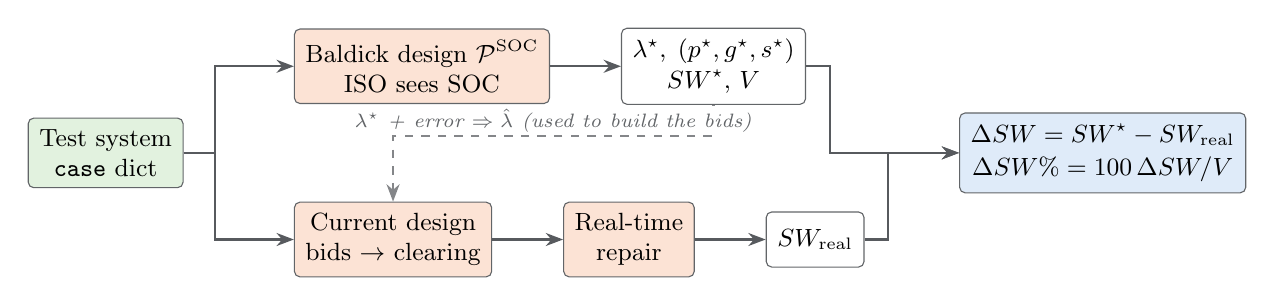
\begin{tikzpicture}[node distance=6mm and 9mm]
  \node[datbox] (case) {Test system\\\code{case} dict};
  \node[lpbox, right=14mm of case, yshift=11mm] (soc) {Baldick design $\mathcal P^{\text{SOC}}$\\ISO sees SOC};
  \node[box, right=of soc] (star) {$\lamstar,\;(p^\star,g^\star,s^\star)$\\$SW^\star$, $V$};
  \node[lpbox, right=14mm of case, yshift=-11mm] (cd) {Current design\\bids $\to$ clearing};
  \node[lpbox, right=of cd] (rt) {Real-time\\repair};
  \node[box, right=of rt] (real) {$SW_{\text{real}}$};
  \node[box, fill=accent!15, right=12mm of real, yshift=11mm, minimum height=10mm] (dsw)
        {$\Delta SW = SW^\star - SW_{\text{real}}$\\[1pt]$\Delta SW\% = 100\,\Delta SW/V$};
  \draw[arr] (case.east) -- ++(4mm,0) |- (soc.west);
  \draw[arr] (case.east) -- ++(4mm,0) |- (cd.west);
  \draw[arr] (soc) -- (star);
  \draw[arr] (cd) -- (rt);
  \draw[arr] (rt) -- (real);
  \draw[arr] (star.east) -- ++(3mm,0) |- (dsw.west);
  \draw[arr] (real.east) -- ++(3mm,0) |- (dsw.west);
  \draw[darr] (star.south) -- ++(0,-4mm) -| node[lab, pos=0.25, above] {$\lamstar$ + error $\Rightarrow \lamhat$ (used to build the bids)} (cd.north);
\end{tikzpicture}
\end{center}

Three facts to keep in mind throughout:
\begin{enumerate}
  \item \textbf{The welfare yardstick is the same function} for the benchmark and for the realised outcome
    (generation cost, redispatch premium, load shedding at VOLL, battery degradation, minus the terminal
    value $w\,s_T$). Only the dispatch it is evaluated at changes.
  \item \textbf{The error enters in one place only}: the price vector the battery uses to build its own bid
    (family \code{B\_fcst}). The system data, the clearing and the welfare evaluation always use the
    \emph{true} parameters.
  \item \textbf{The benchmark is solved once per test system}; each experiment draw solves only the battery's
    own small problems, the hourly clearing and the real-time repair.
\end{enumerate}

% =====================================================================
\section{Repository map and dependencies}
% =====================================================================

\begin{center}
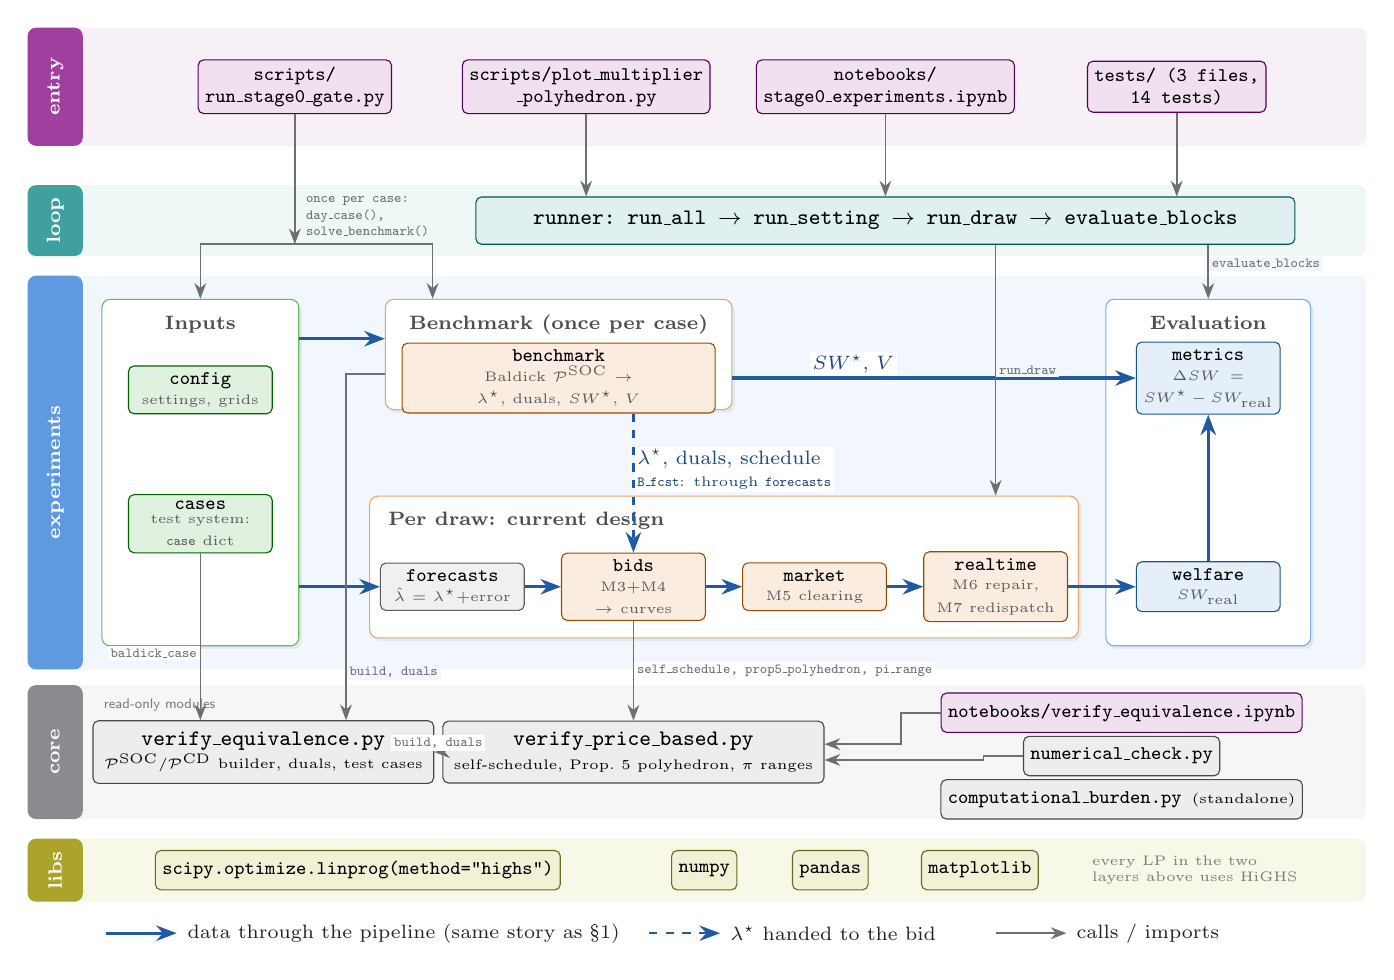
\begin{tikzpicture}[
  lane/.style={draw=none, rounded corners=3pt, minimum width=17cm, anchor=west},
  tab/.style={rounded corners=3pt, minimum width=7mm, anchor=west, text=white, font=\scriptsize\bfseries},
  card/.style={draw=ink!25, fill=white, rounded corners=3pt, drop shadow={opacity=0.12, shadow xshift=0.4mm, shadow yshift=-0.4mm}},
  chip/.style={draw=#1!70!black, fill=#1!12, rounded corners=2pt, font=\ttfamily\scriptsize, inner sep=2.5pt, minimum height=5mm},
  ctitle/.style={font=\scriptsize\bfseries, text=ink!80},
  csub/.style={font=\tiny, text=ink!60},
  imp/.style={-{Stealth[length=2mm]}, semithick, ink!65},
  ilab/.style={font=\tiny\ttfamily, text=ink!65, fill=white, inner sep=1pt},
]
\colorlet{cE}{violet}\colorlet{cO}{teal}\colorlet{cX}{accent}\colorlet{cC}{ink!70}\colorlet{cL}{olive}
\colorlet{cD}{green!55!black}\colorlet{cP}{orange!85!black}\colorlet{cV}{accent}\colorlet{cF}{ink!55}
\tikzset{
  mod2/.style={chip=#1, align=center, text width=1.65cm, font=\ttfamily\scriptsize},
  flow/.style={-{Stealth[length=2.6mm]}, line width=1.2pt, accent!75!black},
  dflow/.style={flow, dashed, line width=0.9pt},
  flab/.style={font=\scriptsize, text=accent!60!black, fill=white, inner sep=1pt},
}
\providecommand{\subt}{\rmfamily\tiny\color{ink!75}}
% ---- lanes ----
\foreach \y/\h/\c/\t in {-0.85/1.5/cE/entry, -2.55/0.9/cO/loop, -5.75/5.0/cX/experiments, -9.3/1.7/cC/core, -10.8/0.8/cL/libs} {
  \node[lane, fill=\c!6, minimum height=\h cm] at (0,\y) {};
  \node[tab, fill=\c!75, minimum height=\h cm] at (0,\y) {\rotatebox{90}{\t}};
}
% ---- entry points ----
\node[chip=cE, align=center] (gate) at (3.4,-0.85) {scripts/\\run\_stage0\_gate.py};
\node[chip=cE, align=center] (plot) at (7.1,-0.85) {scripts/plot\_multiplier\\\_polyhedron.py};
\node[chip=cE, align=center] (snb) at (10.9,-0.85) {notebooks/\\stage0\_experiments.ipynb};
\node[chip=cE, align=center] (tst) at (14.6,-0.85) {tests/ (3 files,\\14 tests)};
% ---- loop ----
\node[chip=cO, minimum width=10.4cm, minimum height=6mm, font=\ttfamily\footnotesize] (run) at (10.9,-2.55)
  {runner:\ run\_all $\to$ run\_setting $\to$ run\_draw $\to$ evaluate\_blocks};
% ---- experiments, laid out as the big picture of Section 1 ----
% inputs
\node[card, draw=cD!60, minimum width=2.5cm, minimum height=4.4cm] (tcard) at (2.2,-5.75) {};
\node[ctitle, anchor=north] at ($(tcard.north)+(0,-0.1)$) {Inputs};
\node[mod2=cD] (cfg) at (2.2,-4.7) {config\\[-1pt]{\subt{} settings, grids}};
\node[mod2=cD] (cas) at (2.2,-6.4) {cases\\[-1pt]{\subt{} test system:\\\texttt{case} dict}};
% benchmark (top row)
\node[card, draw=cP!60, minimum width=4.4cm, minimum height=1.4cm] (bcard) at (6.75,-4.25) {};
\node[ctitle, anchor=north] at ($(bcard.north)+(0,-0.08)$) {Benchmark (once per case)};
\node[chip=cP, align=center, text width=3.8cm, font=\ttfamily\scriptsize] (ben) at (6.75,-4.55)
  {benchmark\\[-1pt]{\subt{} Baldick $\mathcal P^{\text{SOC}}$ $\to$ $\lambda^\star$, duals, $SW^\star$, $V$}};
% one draw of the current design (bottom row)
\node[card, draw=cP!60, minimum width=9.0cm, minimum height=1.8cm] (pcard) at (8.85,-6.95) {};
\node[ctitle, anchor=north west] at ($(pcard.north west)+(0.12,-0.08)$) {Per draw: current design};
\node[mod2=cF] (fc)  at (5.4,-7.2) {forecasts\\[-1pt]{\subt{} $\hat\lambda=\lambda^\star+$error}};
\node[mod2=cP] (bid) at (7.7,-7.2) {bids\\[-1pt]{\subt{} M3+M4 $\to$ curves}};
\node[mod2=cP] (mk)  at (10.0,-7.2) {market\\[-1pt]{\subt{} M5 clearing}};
\node[mod2=cP] (rt)  at (12.3,-7.2) {realtime\\[-1pt]{\subt{} M6 repair, M7 redispatch}};
% evaluation
\node[card, draw=cV!60, minimum width=2.6cm, minimum height=4.4cm] (ecard) at (15.0,-5.75) {};
\node[ctitle, anchor=north] at ($(ecard.north)+(0,-0.1)$) {Evaluation};
\node[mod2=cV] (me) at (15.0,-4.55) {metrics\\[-1pt]{\subt{} $\Delta SW=SW^\star-SW_{\text{real}}$}};
\node[mod2=cV] (wf) at (15.0,-7.2) {welfare\\[-1pt]{\subt{} $SW_{\text{real}}$}};
% ---- data flow (thick): the same story as the big picture ----
\coordinate (bin) at ($(bcard.west)+(0,0.2)$);
\coordinate (bout) at ($(bcard.west)+(0,-0.25)$);
\draw[flow] (bin -| tcard.east) -- (bin);
\draw[flow] (tcard.east |- fc.west) -- (fc.west);
\draw[flow] (fc) -- (bid); \draw[flow] (bid) -- (mk); \draw[flow] (mk) -- (rt);
\draw[flow] (rt) -- (wf);
\draw[flow] (wf) -- (me);
\draw[flow] (bcard.east |- me.west) -- node[flab, above, pos=0.3]{$SW^\star$, $V$} (me.west);
\draw[dflow] (ben.south -| bid.north) -- node[flab, right, pos=0.4, align=left]{$\lambda^\star$, duals, schedule\\{\tiny\code{B\_fcst}: through \code{forecasts}}} (bid.north);
% ---- verified core ----
\node[chip=cC, align=center, font=\ttfamily\footnotesize, inner sep=4pt] (ve) at (3.0,-9.3)
  {verify\_equivalence.py\\[-1pt]{\rmfamily\tiny $\mathcal P^{\text{SOC}}$/$\mathcal P^{\text{CD}}$ builder, duals, test cases}};
\node[chip=cC, align=center, font=\ttfamily\footnotesize, inner sep=4pt] (vpb) at (7.7,-9.3)
  {verify\_price\_based.py\\[-1pt]{\rmfamily\tiny self-schedule, Prop.~5 polyhedron, $\pi$ ranges}};
\node[chip=cE, align=center] (vnb) at (13.9,-8.8) {notebooks/verify\_equivalence.ipynb};
\node[chip=cC, align=center] (nc) at (13.9,-9.35) {numerical\_check.py};
\node[chip=cC, align=center] (cb) at (13.9,-9.9) {computational\_burden.py\ {\rmfamily\tiny(standalone)}};
\node[font=\tiny, text=ink!60, anchor=north west] at (0.85,-8.5) {\textsf{read-only modules}};
% ---- libraries ----
\node[chip=cL] (lp) at (4.2,-10.8) {scipy.optimize.linprog(method="highs")};
\node[chip=cL] at (8.6,-10.8) {numpy};
\node[chip=cL] at (10.2,-10.8) {pandas};
\node[chip=cL] at (12.1,-10.8) {matplotlib};
\node[csub, anchor=west, align=left] at (13.4,-10.8) {every LP in the two\\layers above uses HiGHS};
% ---- calls and imports (thin) ----
\foreach \e in {plot, snb, tst} \draw[imp] (\e.south) -- (\e.south |- run.north);
\draw[imp] (gate.south) -- (3.4,-2.85) coordinate (g0);
\draw[imp] (g0) -| (tcard.north);
\draw[imp] (g0) -| ([xshift=-1.6cm]bcard.north);
\node[ilab, fill=cO!6, anchor=west, align=left] at (3.5,-2.5) {once per case:\\day\_case(),\\solve\_benchmark()};
\draw[imp] (run.south -| rt.north) -- (rt.north |- pcard.north) node[ilab, pos=0.5, right, fill=cX!6]{run\_draw};
\draw[imp] (run.south -| ecard.north) -- (ecard.north) node[ilab, pos=0.35, right, fill=cX!6]{evaluate\_blocks};
\draw[imp] (cas.south) -- (cas.south |- ve.north) node[ilab, pos=0.6, left]{baldick\_case};
\draw[imp] (bout) -| ($(ve.north)+(1.05,0)$) node[ilab, pos=0.93, right, fill=cX!6]{build, duals};
\draw[imp] (bid.south) -- (bid.south |- vpb.north) node[ilab, pos=0.5, right, align=left]{self\_schedule, prop5\_polyhedron, pi\_range};
\draw[imp] (vpb.west) -- (ve.east) node[ilab, midway, above]{build, duals};
\draw[imp] (nc.west) -- ++(-0.5,0) |- ([yshift=-1mm]vpb.east);
\draw[imp] (vnb.west) -- ++(-0.5,0) |- ([yshift=1mm]vpb.east);
% ---- legend ----
\draw[flow] (1.0,-11.6) -- ++(0.9,0) node[right, font=\scriptsize, text=ink]{data through the pipeline (same story as \S1)};
\draw[dflow] (7.9,-11.6) -- ++(0.9,0) node[right, font=\scriptsize, text=ink]{$\lambda^\star$ handed to the bid};
\draw[imp] (12.3,-11.6) -- ++(0.9,0) node[right, font=\scriptsize, text=ink]{calls / imports};
\end{tikzpicture}
\end{center}
{\small Read the experiments layer left to right, like the big picture of \S1: the inputs feed the Baldick
benchmark (top row, solved once by the entry script) and, per draw, the current design (bottom row):
forecast, bid construction, day-ahead clearing, real-time repair. Welfare and $\Delta SW$ close the loop with
$SW^\star$ and $V$ from the benchmark. \code{forecasts} is used only by \code{B\_fcst}; the other bid families
take $\lambda^\star$ (or nothing, \code{B\_priv}) directly. Thin arrows show who calls or imports whom:
\code{runner.run\_draw} drives the bottom row and \code{evaluate\_blocks} runs everything from \code{market}
to \code{welfare}. \code{market}, \code{realtime}, \code{welfare} and \code{metrics} import nothing from the
repository (they receive the \code{case} dict). Not drawn: \code{forecasts} imports \code{config}; the
polyhedron script and the stage-0 notebook also call experiment modules and \code{verify\_price\_based}
directly; the verification notebook and \code{numerical\_check} import both core modules.}

\begin{center}\small
\begin{tabularx}{\textwidth}{@{}l>{\raggedright\arraybackslash}X>{\raggedright\arraybackslash}p{4.3cm}@{}}
\toprule
File & What it contains & Main public objects \\
\midrule
\code{verify\_equivalence.py} & The LP builder shared by both designs; dual extraction with the thesis sign convention; the KKT and Prop.~1--2 checks. \textbf{Read-only.} & \code{baldick\_case}, \code{one\_bus\_case}, \code{LP}, \code{build}, \code{duals}, \code{verify} \\
\code{verify\_price\_based.py} & The battery's own self-schedule LP; the polyhedron of admissible multipliers (Prop.~5); ranges of $\pi_t$. \textbf{Read-only.} & \code{self\_schedule}, \code{prop5\_polyhedron}, \code{pi\_range}, \code{dual\_face\_range} \\
\code{numerical\_check.py} & Re-runs every proposition on Baldick's three cases and writes the thesis figures/table. & \code{run\_case} \\
\code{computational\_burden.py} & Standalone timing benchmark SOC vs.\ CD (own sparse builder, random instances). & \code{instance}, \code{build}, \code{run} \\
\midrule
\code{experiments/config.py} & Frozen dataclasses for one experiment setting, and all stage grids. & \code{ErrorModel}, \code{BidRule}, \code{RealTime}, \code{RunSettings}, \code{stage0\_settings()}, \code{stage1\_settings()} \\
\code{experiments/cases.py} & Test systems. & \code{day\_case}, \code{baldick\_cases}, \code{fleet\_case} (not implemented) \\
\code{experiments/benchmark.py} & Solves $\mathcal P^{\text{SOC}}$ once and the no-storage system; keeps prices, duals, the battery and generator schedules. & \code{solve\_benchmark} $\to$ \code{Benchmark} (\code{lam\_star}, \code{pi\_star}, \code{p/g/s\_star}, \code{q\_star}, \code{SW\_star}, \code{V}) \\
\code{experiments/forecasts.py} & The AR(1) common/specific price-error model. & \code{forecast\_prices}, \code{ar1\_unit\_variance} \\
\code{experiments/bids.py} & The four bid families and the two-block quantity rule. & \code{bid\_star}, \code{bid\_star\_p}, \code{bid\_fcst}, \code{bid\_priv}, \code{quantity\_blocks} \\
\code{experiments/market.py} & Day-ahead clearing of the current design, hour by hour. & \code{clear\_cd}, \code{clear\_hour} \\
\code{experiments/realtime.py} & SOC-feasible repair of the battery schedule; generator redispatch. & \code{feasible\_schedule}, \code{redispatch\_hour} \\
\code{experiments/welfare.py} & Realised welfare and battery profit. & \code{realised\_welfare}, \code{ess\_profit\_day\_ahead} \\
\code{experiments/metrics.py} & $\Delta SW$, decomposition, $\sigma^\star$, summaries. & \code{dsw}, \code{decompose}, \code{sigma\_star}, \code{summarize} \\
\code{experiments/runner.py} & The loop: one row per draw, one CSV per setting, \code{meta.json}. \code{evaluate\_blocks} runs everything after bid construction and returns every intermediate result. & \code{run\_draw}, \code{evaluate\_blocks} $\to$ \code{Outcome} (\code{da}, \code{p/g/s\_rt}, \code{q\_rt}, \code{shed\_rt}, \code{welfare}), \code{run\_setting}, \code{run\_all} \\
\midrule
\code{scripts/run\_stage0\_gate.py} & Runs the stage-0 settings, writes \code{results/stage0/}, asserts the gate. & \code{main} \\
\code{scripts/plot\_multiplier\_polyhedron.py} & Figures of the multiplier polyhedron (\S\ref{sec:poly}). & \code{projection}, \code{fig\_true}, \code{fig\_forecast}, \code{fig\_3d} \\
\code{notebooks/stage0\_experiments.ipynb} & Every step shown on one draw, the interactive explorer and the albums (\S\ref{sec:see}). & \code{simulate\_draw}, \code{draw\_panels}, \code{render\_album} \\
\code{docs/figures/album\_seed1036.html} & Standalone album page: one slider per error parameter, opens without Python. & -- \\
\bottomrule
\end{tabularx}
\end{center}

% =====================================================================
\section{Where the model is created: the \code{case} dictionary}
% =====================================================================

There is no model class. A test system is a plain Python \code{dict}; every LP is \emph{assembled from it on
the fly} by the function that needs it. \code{cases.day\_case()} simply returns
\code{verify\_equivalence.baldick\_case(smax=800, w=40)} (the pilot's own \code{day\_case} is not in the
repository; this substitution is documented in \code{cases.py} and the README).

\begin{center}
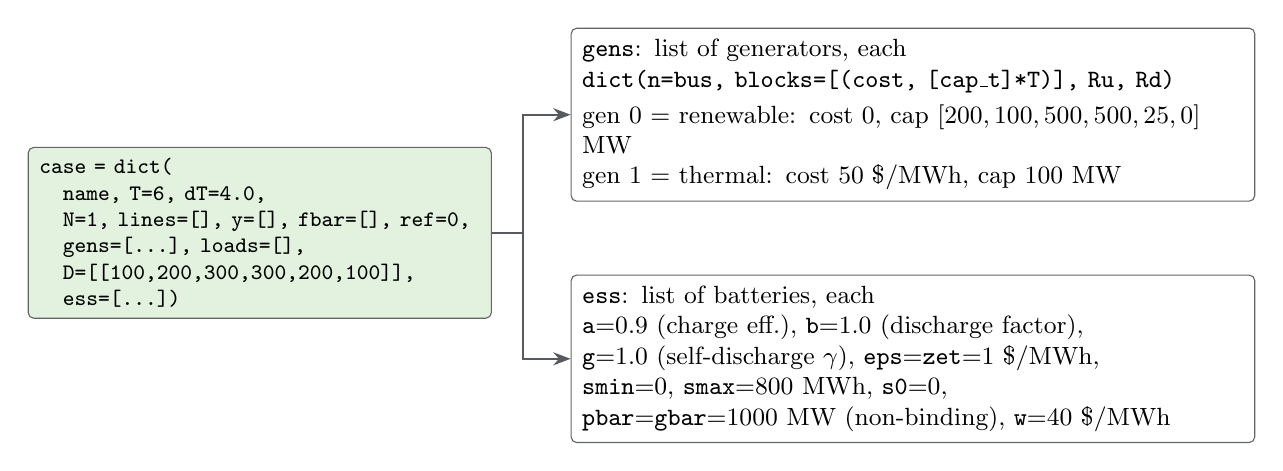
\begin{tikzpicture}[font=\small]
  \node[datbox, align=left, text width=5.6cm, font=\footnotesize] (top) {\code{case = dict(}\\
   \quad \code{name, T=6, dT=4.0,}\\
   \quad \code{N=1, lines=[], y=[], fbar=[], ref=0,}\\
   \quad \code{gens=[...], loads=[],}\\
   \quad \code{D=[[100,200,300,300,200,100]],}\\
   \quad \code{ess=[...])}};
  \node[box, align=left, right=10mm of top, yshift=15mm, text width=8.4cm] (gens) {\textbf{\code{gens}}: list of generators, each\\
    \code{dict(n=bus, blocks=[(cost, [cap\_t]*T)], Ru, Rd)}\\[2pt]
    gen 0 = renewable: cost 0, cap $[200,100,500,500,25,0]$ MW\\
    gen 1 = thermal: cost 50 \$/MWh, cap 100 MW};
  \node[box, align=left, right=10mm of top, yshift=-16mm, text width=8.4cm] (ess) {\textbf{\code{ess}}: list of batteries, each\\
    \code{a}=0.9 (charge eff.), \code{b}=1.0 (discharge factor),\\
    \code{g}=1.0 (self-discharge $\gamma$), \code{eps}=\code{zet}=1 \$/MWh,\\
    \code{smin}=0, \code{smax}=800 MWh, \code{s0}=0,\\
    \code{pbar}=\code{gbar}=1000 MW (non-binding), \code{w}=40 \$/MWh};
  \draw[arr] (top.east) -- ++(4mm,0) |- (gens.west);
  \draw[arr] (top.east) -- ++(4mm,0) |- (ess.west);
\end{tikzpicture}
\end{center}

\begin{itemize}
  \item \textbf{Time}: $T=6$ intervals of $\Delta T = 4$\,h (one day). Powers are MW, energies MWh, so every
    power term carries a factor \code{dT} when it enters an energy balance or a cost.
  \item \textbf{Renewables} are a zero-cost generator with a time-varying capacity. Curtailment is therefore
    implicit: the LP simply dispatches less than the cap (this is what happens at $t=3,4$, where
    $\lamstar=0$).
  \item \textbf{Demand} is inelastic (\code{loads=[]}), so welfare reduces to minus total cost.
  \item \textbf{Load shedding} is not a variable of \code{build}. \code{benchmark.with\_shedding\_generator}
    adds a generator priced at VOLL $=1000$ \$/MWh (capacity $2\times$ peak demand); \code{market} and
    \code{realtime} add an explicit shedding column priced at VOLL.
\end{itemize}
\begin{center}
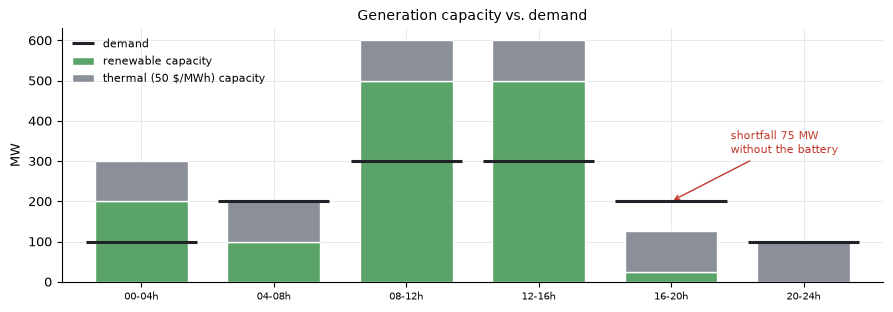
\includegraphics[width=0.78\textwidth]{figures/nb_capacity.png}\\[-1pt]
{\footnotesize Generation capacity against demand (notebook \S1): without storage, 16--20h is 75\,MW short.}
\end{center}

% =====================================================================
\section{The optimisation models}
% =====================================================================

Seven LP families are solved, all with SciPy \code{linprog(method="highs")}. The table locates each one; the
subsections give the abstract model.

\begin{center}\small
\begin{tabularx}{\textwidth}{@{}c>{\raggedright\arraybackslash}p{3.2cm}>{\raggedright\arraybackslash}X>{\raggedright\arraybackslash}p{2.9cm}c@{}}
\toprule
& Model & Built in & Called by & per draw \\
\midrule
M1 & $\mathcal P^{\text{SOC}}$ Baldick clearing & \code{verify\_equivalence.build(case,"SOC")} & \code{benchmark} & once/case \\
M2 & $\mathcal P^{\text{CD}}$ single-block clearing & \code{verify\_equivalence.build(case,"CD",bids)} & verification only & -- \\
M3 & $\mathcal P^{\text{SS}}(\lambda)$ self-schedule & \code{verify\_price\_based.self\_schedule} & \code{bids} & 1 \\
M4 & Prop.~5 polyhedron $\Pi$: range / vertex & \code{verify\_price\_based.pi\_range}, \code{bids.\_solver\_vertex} & \code{bids} & $2T$ or 1 \\
M5 & Hourly day-ahead clearing & \code{market.clear\_hour} & \code{runner} & $T$ \\
M6 & SOC-feasible repair (L1) & \code{realtime.feasible\_schedule} & \code{runner} & 1 per ESS \\
M7 & Hourly redispatch & \code{realtime.redispatch\_hour} & \code{runner} & $T$ \\
\bottomrule
\end{tabularx}
\end{center}

\subsection{M1 -- Baldick's SOC design $\mathcal P^{\text{SOC}}$ (the benchmark)}
\label{sec:soc}
Indices: generator $i$, block $k$, battery $e$, bus $n$, interval $t$. In the single-bus case the flow,
angle and ramp rows exist in the code but are empty or non-binding.
\begin{align*}
\min\;& \sum_t \Delta T\Big[\sum_{i,k} c_{ik} q_{ikt} - \sum_{m,j} U_{mj} d_{mjt}
       + \sum_e(\varepsilon_e p_{et} + \zeta_e g_{et})\Big] - \sum_e w_e s_{eT} \\
\text{s.t.}\;
& \textstyle\sum d_{nt} + D_{nt} + \sum_l A_{nl} f_{lt} - \sum q_{nt} - \sum_{e\in n}(g_{et} - p_{et}) = 0
  && [\lambda_{nt}] && \text{(A1) balance}\\
& f_{lt} = y_l \textstyle\sum_n A_{nl}\theta_{nt},\quad \theta_{\text{ref},t}=0 && [\kappa,\xi] && \text{(A2),(A4)}\\
& -R^d_i \le \textstyle\sum_k q_{ikt} - \sum_k q_{ik,t-1} \le R^u_i && [\tau] && \text{(A6) ramps}\\
& s_{et} = \gamma_e s_{e,t-1} + \Delta T\, a_e p_{et} - \Delta T\, b_e g_{et} && [\pi_{et}] && \text{(A8) SOC dynamics}\\
& \gamma_e s_{e,t-1} + \Delta T\, a_e p_{et} \le \bar s_e && [\nuU_{et}] && \text{(A9) upper SOC}\\
& \gamma_e s_{e,t-1} - \Delta T\, b_e g_{et} \ge \underline s_e && [\nuL_{et}] && \text{(A10) lower SOC}\\
& 0\le q\le \bar Q,\; 0\le d\le\bar d,\; |f|\le \bar f,\; 0\le p\le\bar p,\; 0\le g\le \bar g && && \text{(A3,5,7,11,12)}
\end{align*}
(A9)/(A10) bound the SOC reached by charging alone and by discharging alone, which is the same as
$\underline s\le s_t\le\bar s$ whenever the battery does not charge and discharge in the same interval.
The constant $w_e\gamma_e^T s_{e0}$ of the terminal value is dropped in the LP and added back in
\code{benchmark.solve\_benchmark}: $SW^\star = -(f^{\text{SOC}\star} + \sum_e w_e\gamma_e^T s_{e0})$.

\textbf{Dual extraction} (\code{verify\_equivalence.duals}). SciPy returns $\partial f^\star/\partial\text{rhs}$.
With the note's Lagrangian $L=f+y(\text{lhs}-\text{rhs})$: equality and $\le$ rows give $y=-\text{marginal}$,
upper bounds $\bar y = -\text{upper.marginal}/\Delta T$, lower bounds $\underline y=\text{lower.marginal}/\Delta T$;
power rows (tags \code{lam, kap, xi, tauU, tauL}) are divided by $\Delta T$ so every multiplier is in \$/MWh.
The result is a dict keyed by row tag, e.g.\ \code{y["pi", e, t]}.

\textbf{KKT rows used later.} Stationarity in $p$, $g$, $s$:
\[
\varepsilon + \lambda_t - a(\pi_t - \nuU_t) + \bar\rho_t - \underline\rho_t = 0,\qquad
\zeta - \lambda_t + b(\pi_t + \nuL_t) + \bar\sigma_t - \underline\sigma_t = 0,
\]
\[
\pi_t = \gamma\,(\pi_{t+1} - \nuU_{t+1} + \nuL_{t+1}),\qquad \pi_T = w .
\]
So $\pi_t$ is the marginal value of stored energy, propagated backwards from the terminal value $w$, with a
jump wherever an SOC limit binds.

\subsection{M2 -- Current design $\mathcal P^{\text{CD}}$ and the equivalent bids (E)}
Same LP with $s$ and (A8)--(A10) removed; the battery's cost term becomes its bid:
\[
\textstyle\sum_t\Delta T\,(-u_{et}\,p_{et} + c_{et}\,g_{et}),\qquad
\boxed{u_{et} = a_e(\pi_{et}-\nuU_{et}) - \varepsilon_e,\qquad c_{et} = \zeta_e + b_e(\pi_{et}+\nuL_{et})}\quad\text{(E)}
\]
Substituting (E) into the KKT rows above shows that $(x^\star,\lamstar)$ satisfies the KKT conditions of
$\mathcal P^{\text{CD}}$: this is Theorem~1. M2 is only used by the verification scripts; the experiments use
the multi-block version M5.

\subsection{M3 -- The battery's self-schedule $\mathcal P^{\text{SS}}_e(\lambda)$, with a tie-breaker}
\label{sec:m3}
The battery alone, as a price-taker against a price vector $\lambda$ (true \emph{or} forecast). Its true
objective (minus its profit) is
\[
f(p,g,s;\lambda)=\sum_t \Delta T\big[(\varepsilon+\lambda_t)p_t + (\zeta-\lambda_t)g_t\big] - w\,s_T ,
\]
and the plan the experiments use solves
\[
\boxed{\;\min_{p,g,s}\; f(p,g,s;\lambda)\;-\;\kappa\sum_t \Delta T\,(p_t+g_t)
\quad\text{s.t. (A8)--(A12) of battery } e\;}
\]
with $\kappa=10^{-3}$\,\$/MWh (\code{BidRule.tie\_break\_reward}).
Lemma~4: at $\lambda=\lamstar$ Baldick's schedule is optimal for $f$. Output: a planned schedule
$(p^\circ, g^\circ, s^\circ)$, used both as the \emph{quantity} of the bid and to define M4.

\textbf{What the extra term does.} It rewards throughput $\sum_t\Delta T(p_t+g_t)$, the MWh the battery
trades, with $\kappa$ per MWh. $\kappa$ is far below any real profit difference, so it never makes the battery
give up profit: it only decides between plans that earn \emph{exactly} the same. In words: \emph{among all
plans that maximise the battery's true profit, take the one that trades the most.} The code enforces this
strictly (\code{bids.self\_schedule}): it checks that the plan's true objective $f$ equals the optimum of
$f$ (to $10^{-9}$ relative) and halves $\kappa$ until it does. So the plan is always optimal for the true
problem, and everything built on that (Lemma~4, the polyhedron $\Pi$ of M4, Theorem~1) still holds. The term
appears only here. Welfare (M7) is computed from the realised dispatch at the true costs, so $\kappa$ never
enters $SW$ or $\Delta SW$. $\kappa=0$ switches the tie-breaker off.

\emph{Implementation:} the term only changes the objective, and it equals running the unchanged
self-schedule LP (\code{verify\_price\_based}) with $\varepsilon\to\varepsilon-\kappa$ and $\zeta\to\zeta-\kappa$.
Those two parameters appear nowhere else in that LP, so its constraints are reused, not copied. An assert keeps
$2\kappa<\varepsilon+\zeta$, so simultaneous charging and discharging can never look free.

\textbf{Why we apply it.} At the true prices the battery is indifferent between many plans, because
$\lamstar$ is full of ties: a break-even round trip at 00--08h ($(43.1+\varepsilon)/\alpha=49=50-\zeta$), two
free intervals at 08--16h (both priced 0) and two evening intervals at 50. Without a rule, the plan is
whichever optimal vertex the LP solver happens to return. That is an artefact of the algorithm, not a
decision of the owner, and it can change with the solver, its version or the order of the constraints. The
tie-breaker replaces that accident with a stated, economically sensible rule: a battery that is indifferent
offers its capacity to the market rather than holding it back.
\begin{center}\small
\begin{tabular}{@{}lccc@{}}
\toprule
Self-schedule at $\lamstar$ & plan $p^\circ$ / $g^\circ$ (MW, 6 intervals) & throughput & \code{B\_star\_p} loss \\
\midrule
$\kappa=0$ (solver's vertex) & $p^\circ=(0,0,0,222,0,0)$, $g^\circ=(0,0,0,0,200,0)$ & 1\,689 MWh & 6.32\,\% of $V$\\
$\kappa=10^{-3}$ (tie-breaker) & $p^\circ=(222,0,0,222,0,0)$, $g^\circ=(0,200,0,0,0,200)$ & 3\,378 MWh & \textbf{1.30}\,\% of $V$\\
\bottomrule
\end{tabular}
\end{center}
The solver's vertex skips the morning round trip, because at break-even it earns nothing. The tie-broken plan
runs it (buy at 00--04h, sell at 04--08h), as Baldick's schedule does, so the zero-error loss is 1.30\% of
$V$ instead of 6.32\%.

\textbf{What it does not do.} (i) It breaks only \emph{exact} ties. Any forecast error makes one plan strictly
better, and the tie-breaker then has nothing to choose. It changed the plan in 0 of the 750 forecast draws of
stage~0, so it moves only the $\sigma=0$ numbers. (ii) It cannot break a \emph{timing} tie, where two plans
trade the same MWh at different times (buy the free energy at 08--12h or at 12--16h; sell at 16--20h or at
20--24h). The remaining 1.30\% is exactly such a tie: the plan buys all 222\,MW at 12--16h, where only
200\,MW of free energy exists, while Baldick's schedule also buys at 08--12h. The battery ends up with 80\,MWh
less stored and 100\,MWh more thermal energy is burned (+5\,000\,\$). Adding +400\,\$ of redispatch,
$-800$\,\$ for the 20\,MWh left at the end and $-189$\,\$ of degradation gives 4\,411\,\$ $=1.30\%$ of $V$.
(iii) A larger $\kappa$ that deliberately gives up profit for activity would act on \emph{near}-ties too.
That would be a behavioural assumption, not a tie-breaker, and is not used.

\subsection{M4 -- The multiplier polyhedron $\Pi$ (Prop.~5) and the selection rule}
Given $\lambda$ and the planned schedule, the admissible multipliers $x=(\pi,\nuU,\nuL)\in\mathbb R^{3T}$ are
\begin{align*}
&\pi_T = w,\qquad \pi_t = \gamma(\pi_{t+1}-\nuU_{t+1}+\nuL_{t+1}) && \text{(costate)}\\
&\nuU_t \ge 0 \text{ if (A9) is tight at } t,\ \text{else } \nuU_t=0;\quad \text{same for }\nuL_t,\text{(A10)} && \text{(compl.\ slackness)}\\
&u_t \le \lambda_t \text{ if } p^\circ_t=0,\quad u_t\ge\lambda_t \text{ if } p^\circ_t=\bar p,\quad u_t=\lambda_t \text{ otherwise} && \text{(price consistency)}\\
&c_t \ge \lambda_t \text{ if } g^\circ_t=0,\quad c_t\le\lambda_t \text{ if } g^\circ_t=\bar g,\quad c_t=\lambda_t \text{ otherwise}
\end{align*}
with $u,c$ from (E). Any point of $\Pi$ gives valid bids; $\Pi$ is generally \emph{not} a single point
(degenerate duals). \code{pi\_range} solves $2T$ LPs ($\min$/$\max\ \pi_t$) to get $[\mathrm{lo}_t,\mathrm{hi}_t]$.
The point is chosen by \code{BidRule.rule}:
\begin{itemize}
  \item \code{"prelimit"} (\code{bids.\_prelimit\_vertex}): $\pi_1=\mathrm{hi}_1$, then
    $\pi_t=\operatorname{clip}(\pi_{t-1}/\gamma,\ \mathrm{lo}_t,\ \mathrm{hi}_t)$; $\nuU,\nuL$ are then solved
    from the costate equation (only one can be non-zero at each $t$).
  \item \code{"solver"} (\code{bids.\_solver\_vertex}): the vertex of $\Pi$ minimising $\sum_t\pi_t$ (one LP).
\end{itemize}

\subsection{From multipliers to a bid curve: the quantity rule}
\code{bids.quantity\_blocks} turns $(u_t,c_t,p^\circ_t,g^\circ_t)$ into two blocks per side with a small spread
$\delta=0.01$ \$/MWh, so the clearing prefers the planned quantity at the price $\lamstar$:
\[
\text{charge: } (u_t+\delta,\ p^\circ_t),\ (u_t-\delta,\ \bar p-p^\circ_t);\qquad
\text{discharge: } (c_t-\delta,\ g^\circ_t),\ (c_t+\delta,\ \bar g-g^\circ_t).
\]
\begin{center}
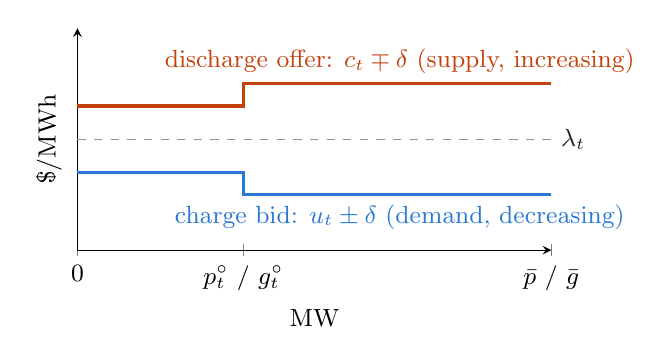
\begin{tikzpicture}
\begin{axis}[width=7.6cm, height=4.4cm, xmin=0, xmax=1000, ymin=36, ymax=56, axis lines=left,
  xlabel={MW}, ylabel={\$/MWh}, xtick={0,350,1000}, xticklabels={0,$p^\circ_t$ / $g^\circ_t$,$\bar p$ / $\bar g$},
  ytick=\empty, label style={font=\small}, tick label style={font=\small}, clip=false]
  \addplot[very thick, accent, const plot] coordinates {(0,43) (350,43) (350,41) (1000,41)};
  \addplot[very thick, warn, const plot] coordinates {(0,49) (350,49) (350,51) (1000,51)};
  \draw[dashed, ink!50] (axis cs:0,46) -- (axis cs:1000,46) node[right, font=\small, text=ink]{$\lambda_t$};
  \node[font=\small, text=accent] at (axis cs:680,39) {charge bid: $u_t\pm\delta$ (demand, decreasing)};
  \node[font=\small, text=warn] at (axis cs:680,53) {discharge offer: $c_t\mp\delta$ (supply, increasing)};
\end{axis}
\end{tikzpicture}
\end{center}
{\small Illustrative prices. The band $[u_t, c_t]$ always contains $\lamstar_t$ (for \code{B\_star}), with
$\lamstar_t$ on an edge whenever the battery is marginal. \code{B\_priv} uses one full-capacity block per
side and no spread.}

The actual bids of the four families on the test system (notebook \S4; \code{B\_fcst} for seed 1005,
$\sigma=1$\,\$/MWh). Blue edge = charge bid $u_t$ (buys if the price is $\le u_t$), orange edge = offer $c_t$
(sells if $\ge c_t$), dot = $\lamstar_t$:
\begin{center}
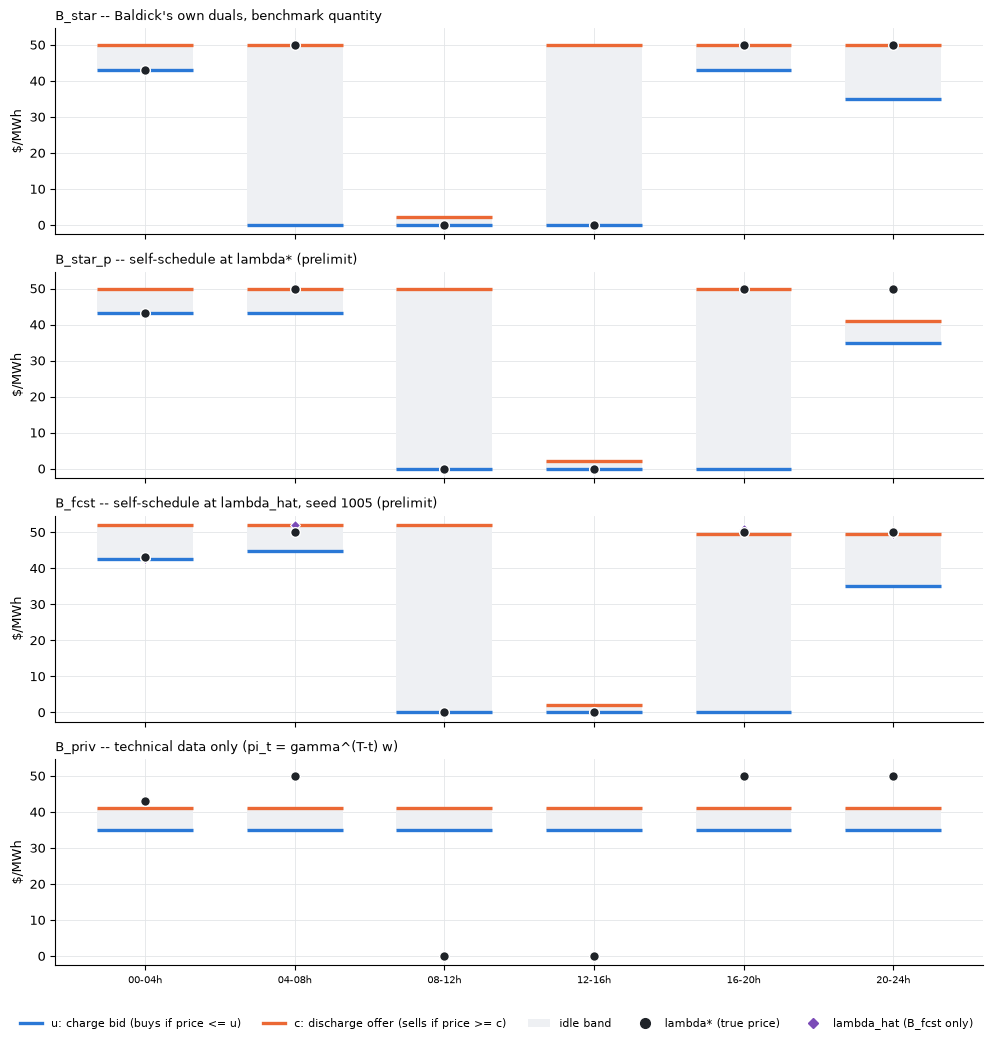
\includegraphics[width=0.8\textwidth]{figures/nb_bid_bands.png}
\end{center}

\subsection{M5 -- Day-ahead clearing of the current design (\code{market.clear\_hour})}
Single bus, one LP per hour $t$ (valid because ramps are non-binding in \code{day\_case}). Generator blocks
$j$ at their true cost $c_j$, each battery's blocks $k$, a shedding column:
\[
\min\ \sum_j c_j q_j - \sum_{e,k} u_{ek}\,x^p_{ek} + \sum_{e,k} c_{ek}\,x^g_{ek} + \text{VOLL}\cdot sh
\quad\text{s.t.}\quad \sum_j q_j - \sum_{e,k}x^p_{ek} + \sum_{e,k}x^g_{ek} + sh = D_t\ \ [\lambda^{\text{CD}}_t]
\]
with $0\le q_j\le\bar Q_{jt}$, $0\le x_{ek}\le$ block size, $0\le sh\le D_t$. There is \textbf{no SOC
constraint}: the result $p^{da}_e=\sum_k x^p_{ek}$, $g^{da}_e=\sum_k x^g_{ek}$ may be physically
infeasible for the battery. Output: \code{DayAheadResult(q\_da, p\_da, g\_da, shed, lam\_cd)}.

Each interval is a merit-order auction (notebook \S7.3, seed 1005, $\sigma=1$): supply = generators + the
battery's offer blocks + shedding, demand = load + the battery's bid blocks; the dot is the cleared point.
\begin{center}
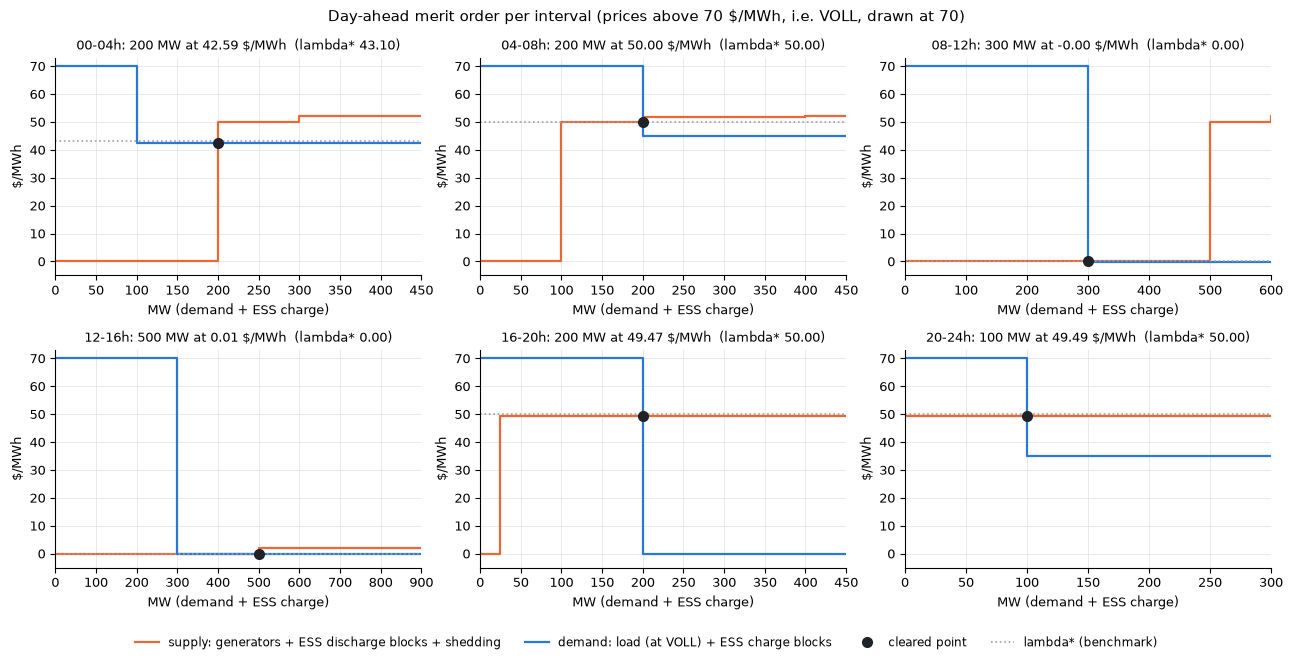
\includegraphics[width=\textwidth]{figures/nb_merit_order.png}
\end{center}
Because no SOC enters the clearing, the accepted schedule can take the battery outside its limits (right
panel: the SOC the day-ahead schedule \emph{would} produce, red $\times$ = infeasible):
\begin{center}
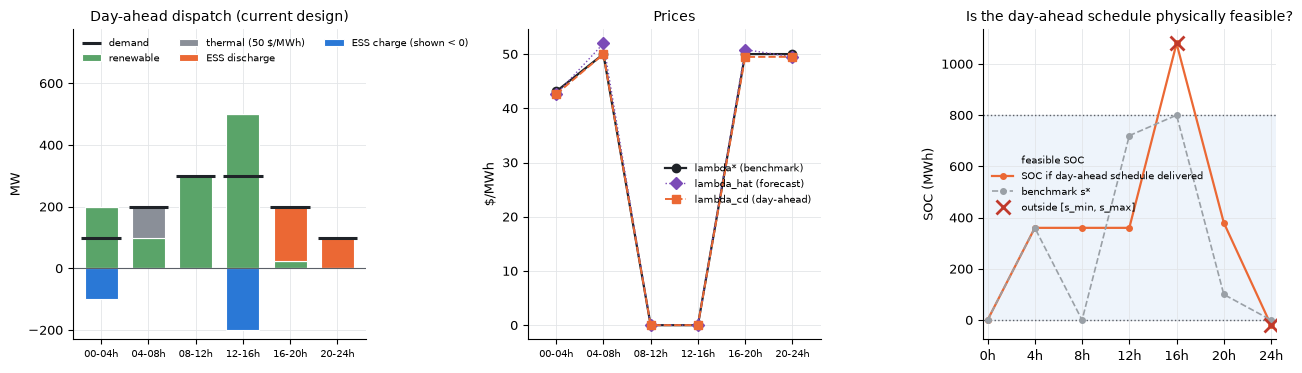
\includegraphics[width=\textwidth]{figures/nb_da_feasibility.png}
\end{center}

\subsection{M6 -- Real-time repair of the battery (\code{realtime.feasible\_schedule})}
The battery delivers the physically feasible schedule closest (L1) to what it sold, with its \emph{true}
parameters:
\[
\min_{p,g,s}\ \sum_t |p_t - p^{da}_t| + |g_t - g^{da}_t|\quad\text{s.t. (A8)--(A12)},
\qquad \text{Undeliverable} = \Delta T\sum_t\big(|p_t-p^{da}_t|+|g_t-g^{da}_t|\big)\ \text{MWh}.
\]
Implemented with the split $p=p^{da}+p^{+}-p^{-}$, $p^{\pm}\ge0$ (same for $g$): $7T$ variables.

\subsection{M7 -- Generator redispatch (\code{realtime.redispatch\_hour})}
Per hour, generators move from $q^{da}$ to cover the net demand left after the battery's real-time action
$N_t = D_t - \sum_e g^{rt}_{et} + \sum_e p^{rt}_{et}$, paying a premium $\psi$ per MWh moved in either direction:
\begin{align*}
\min_{q^+,q^-,sh}\ & \sum_j (c_j+\psi)q^+_j + (\psi-c_j)q^-_j + \text{VOLL}\cdot sh\\
\text{s.t.}\ & \sum_j(q^+_j-q^-_j) + sh = N_t - \sum_j q^{da}_j,\qquad 0\le q^+_j\le\bar Q_{jt}-q^{da}_j,\quad 0\le q^-_j\le q^{da}_j .
\end{align*}
$q^{rt}=q^{da}+q^+-q^-$. Moving down saves $c_j$ but still costs $\psi$.

M6 and M7 on the same draw (notebook \S7.4): what the battery sold vs.\ what it can deliver, the SOC paths
(plan, day-ahead, real time, benchmark), the generator redispatch, and the real-time dispatch.
\begin{center}
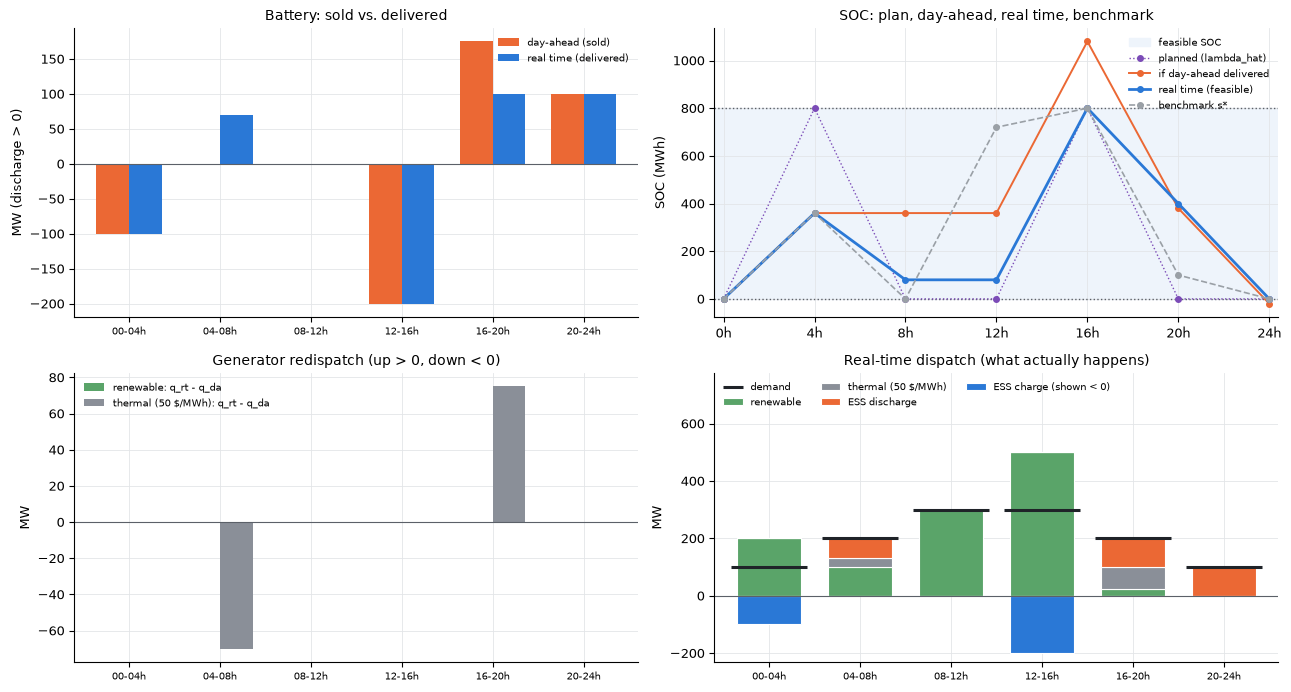
\includegraphics[width=\textwidth]{figures/nb_realtime.png}
\end{center}

\subsection{Welfare and metrics}
\begin{align*}
SW_{\text{real}} &= -\Big(\Delta T\!\sum_{j,t} c_j q^{rt}_{jt} + \psi\,\Delta T\!\sum_{j,t}|q^{rt}_{jt}-q^{da}_{jt}|
 + \text{VOLL}\,\Delta T\!\sum_t sh_t + \Delta T\!\sum_{e,t}(\varepsilon_e p^{rt}_{et}+\zeta_e g^{rt}_{et}) - \sum_e w_e s^{rt}_{eT}\Big)\\
SW_{\text{noESS}} &= -f^\star\big(\mathcal P^{\text{SOC}}\text{ with no battery + VOLL generator}\big),\qquad
V = SW^\star - SW_{\text{noESS}}\ \ (\text{storage value})\\
\Delta SW &= SW^\star - SW_{\text{real}}\ \ (\text{asserted} \ge -10^{-6}),\qquad \Delta SW\% = 100\,\Delta SW/V
\end{align*}
Further metrics (\code{metrics.py}): price distortion $\overline{|\lambda^{\text{CD}}-\lamstar|}$;
decomposition quantity part $=\Delta SW(\code{B\_star\_p})$, price part $=\Delta SW(\code{B\_fcst})-\Delta SW(\code{B\_star\_p})$
(accounting split, not causal); $\sigma^\star$ where mean loss of \code{B\_fcst} crosses that of \code{B\_priv};
mean, 95\% CI, median, p95 per setting. Battery profit is the day-ahead settlement at $\lambda^{\text{CD}}$
minus degradation (real-time costs it causes are not charged to it; flagged assumption).

% =====================================================================
\section{The forecast error}
% =====================================================================

\subsection{Model (\code{forecasts.forecast\_prices})}
For battery $e$ and interval $t$, with $\bar\lambda=\operatorname{mean}(\lamstar)$:
\[
\lamhat_{et} = \max\Big(\underline\lambda,\; \lamstar_t + \underbrace{\tfrac{\text{bias\_pct}}{100}\,\bar\lambda}_{\text{bias}}
 + \sigma\, z_{et}\Big),\qquad
z_{et} = \sqrt{\omega}\,\chi_t + \sqrt{1-\omega}\,\eta_{et},
\]
\[
\sigma = \begin{cases}\text{\code{sigma\_abs}} & \text{if given (\$/MWh)}\\ \tfrac{\text{\code{sigma\_pct}}}{100}\bar\lambda & \text{otherwise}\end{cases}
\]
$\chi$ (common to all batteries) and $\eta_e$ (battery-specific) are independent unit-variance AR(1)
paths, each drawn by \code{ar1\_unit\_variance}:
\[
x_1\sim\mathcal N(0,1),\qquad x_t=\rho\, x_{t-1}+\sqrt{1-\rho^2}\,w_t,\quad w_t\sim\mathcal N(0,1)\text{ i.i.d.},
\]
hence $\operatorname{Var}z=1$, $\operatorname{corr}(z_t,z_{t+1})=\rho$ and
$\operatorname{corr}(z_{e},z_{e'})=\omega$.
With $\sigma=0$ the function returns $\max(\underline\lambda,\lamstar+\text{bias})$ exactly, without touching
the RNG. The \textbf{price floor} $\underline\lambda$ (\code{ErrorModel.price\_floor}, default 0, \code{None}
disables it) keeps the forecast inside the range of prices the market can actually produce
(\S\ref{sec:values}).

\begin{center}
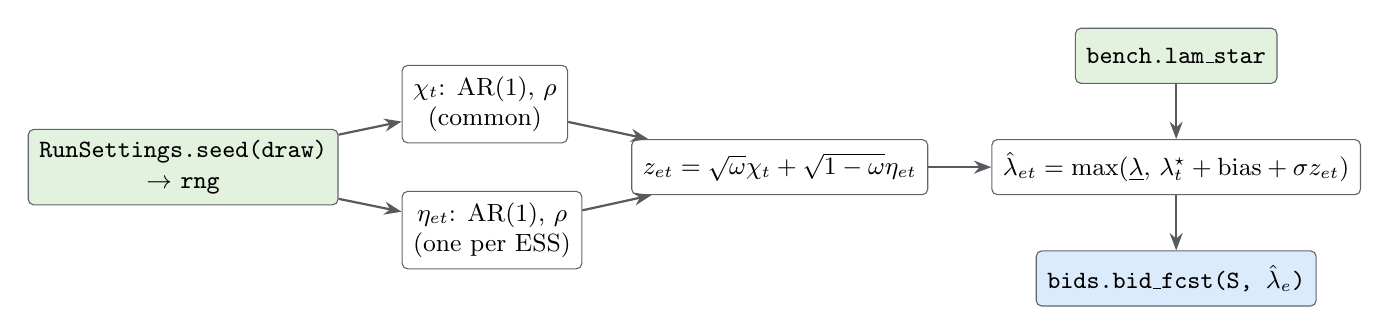
\begin{tikzpicture}[node distance=5mm and 8mm]
  \node[datbox] (seed) {\code{RunSettings.seed(draw)}\\$\to$ \code{rng}};
  \node[box, right=of seed, yshift=8mm] (chi) {$\chi_t$: AR(1), $\rho$\\(common)};
  \node[box, right=of seed, yshift=-8mm] (eta) {$\eta_{et}$: AR(1), $\rho$\\(one per ESS)};
  \node[box, right=of chi, yshift=-8mm] (z) {$z_{et}=\sqrt\omega\chi_t+\sqrt{1-\omega}\eta_{et}$};
  \node[box, right=of z] (lh) {$\lamhat_{et}=\max(\underline\lambda,\,\lamstar_t+\text{bias}+\sigma z_{et})$};
  \node[mod, below=7mm of lh] (bf) {bids.bid\_fcst(S, $\lamhat_e$)};
  \node[datbox, above=7mm of lh] (ls) {\code{bench.lam\_star}};
  \draw[arr] (seed) -- (chi); \draw[arr] (seed) -- (eta);
  \draw[arr] (chi) -- (z); \draw[arr] (eta) -- (z); \draw[arr] (z) -- (lh);
  \draw[arr] (ls) -- (lh); \draw[arr] (lh) -- (bf);
\end{tikzpicture}
\end{center}

\subsection{Seeds: one error shape per draw, shared by every setting}
\label{sec:crn}
To compare error sizes (and, next, bid designs) properly, every setting must face the \emph{same}
forecast-error scenarios. A difference in loss between $\sigma=1$ and $\sigma=5$ should come from the size
of the error alone, not from one setting happening to draw more harmful error shapes than the other. We
therefore derive the seed of draw $d$ from the draw number only,
\[
\code{seed}(d)=\code{SeedSequence}(\code{base\_seed},\,d),
\]
and all randomness of the draw comes from one generator, \code{rng = default\_rng(RunSettings.seed(d))}.
Because the seed does not depend on the setting, draw $d$ uses the same innovations $w_t$, and so the same
$\chi$, $\eta$ and $z$, in every setting that shares \code{base\_seed}. $\sigma$ and the bias only scale and
shift that shape, and $\rho$ and $\omega$ only change how the same innovations are combined. This is the
\textbf{common random numbers} (CRN) design:
\begin{center}\small
\begin{tabular}{@{}lccc@{}}
\toprule
& $\sigma=1$ & $\sigma=5$ & $\sigma=20$ \\
\midrule
draw $d$ & shape A $\times1$ & shape A $\times5$ & shape A $\times20$\\
draw $d+1$ & shape B $\times1$ & shape B $\times5$ & shape B $\times20$\\
\bottomrule
\end{tabular}
\end{center}
A comparison between two settings is then \emph{paired}: both face the same forecast shapes, and the
difference comes from the parameter or the design alone. This also makes the comparison much more precise:
$\operatorname{Var}(\bar L_A-\bar L_B)=\operatorname{Var}\bar L_A+\operatorname{Var}\bar L_B
-2\operatorname{Cov}(\bar L_A,\bar L_B)$, and shared shapes make the covariance large. Since the settings are
not independent samples, the confidence interval of a \emph{difference} is computed from the per-draw
differences (\code{metrics.paired\_difference}), not from the two settings' own intervals. Finally,
\code{SeedSequence} is a fixed function of $(\code{base\_seed},d)$, so every draw can be regenerated in any
session from its number; each result row stores its seed. Stage-0 effect: \S\ref{sec:numbers}.

The same steps on one draw (notebook \S3, seed 1005, $\sigma=1$\,\$/MWh, floor 0): the error shape $z$, the
scaled error, the resulting forecast, and where this draw sits among 500 draws. In the two zero-price
intervals the floor clips the forecast to 0.
\begin{center}
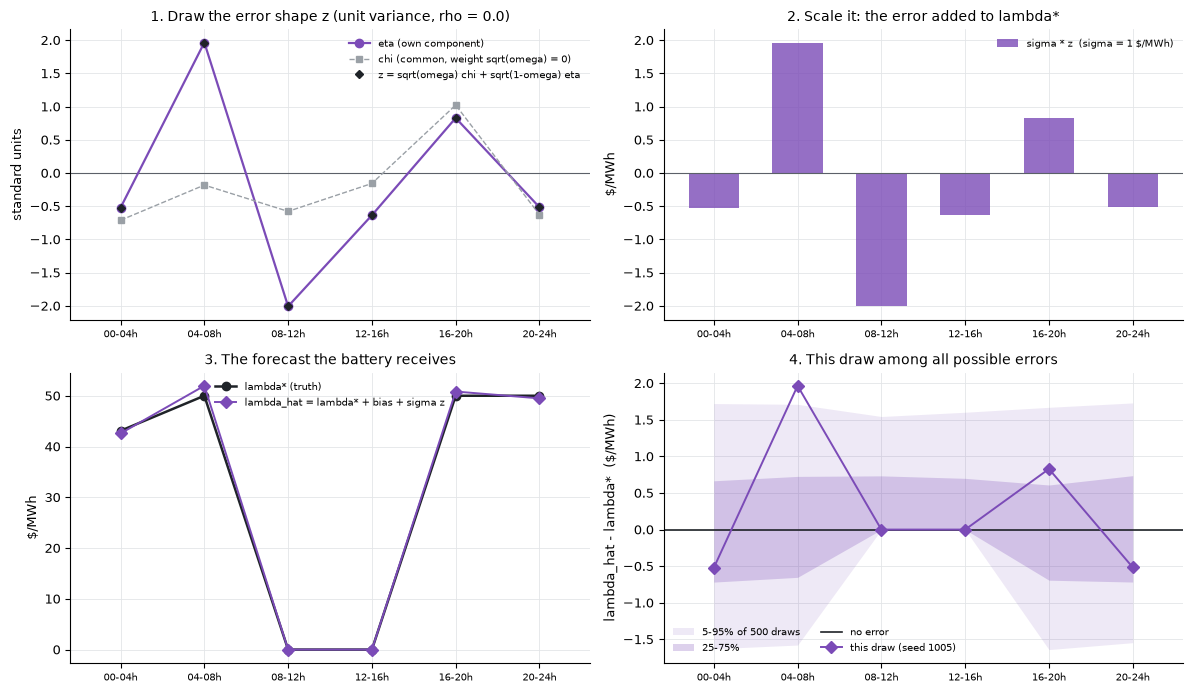
\includegraphics[width=0.9\textwidth]{figures/nb_forecast_steps.png}
\end{center}

\subsection{Where the error is inserted}
Only in \code{runner.run\_draw}, branch \code{family == "B\_fcst"}: $\lamhat_e$ replaces $\lamstar$ as the
input of M3 (self-schedule) \emph{and} M4 (polyhedron). It therefore corrupts both parts of the bid:
\begin{itemize}
  \item the \textbf{quantity} $(p^\circ,g^\circ)$: the battery plans to charge/discharge in the wrong hours;
  \item the \textbf{price} $(u,c)$: the multiplier $\pi$ (value of stored energy) is computed at the wrong prices.
\end{itemize}
Nothing downstream sees $\lamhat$: clearing (M5), repair (M6), redispatch (M7) and welfare use the true
system and true battery parameters. The error is a \emph{price} error, not a renewable or load error: the
system itself is deterministic.

% =====================================================================
\section{Choosing the error values, and how to defend them}
\label{sec:values}
% =====================================================================

The error values are a \textbf{design of experiments, not an estimate}. Each one is chosen by four rules
that can be stated and defended independently of the results:
\begin{enumerate}
  \item \textbf{Scale-free units.} $\sigma$ and the bias are percentages of the mean benchmark price
    $\bar\lambda$, so a result transfers across systems and currencies, and matches how forecast accuracy is
    reported in the literature (relative errors).
  \item \textbf{Bracket reality, include the control.} Each axis runs from \emph{perfect information} (0, the
    control: it must reproduce the zero-error result) to \emph{a naive forecaster}, with the published
    state-of-the-art values in between.
  \item \textbf{Geometric spacing.} Doubling steps resolve small errors finely and still reach poor forecasts
    with few settings.
  \item \textbf{Calibration replaces stylised values.} Stage~3 (\code{experiments.md}, ``Calibration'') backtests
    a naive forecaster on real DK1/DK2 prices and estimates $\sigma$, bias, $\rho$ and $\omega$. The grid's job is
    to show the \emph{shape} of the loss; the calibrated point is then placed on it.
\end{enumerate}

\subsection{Forecast error size $\sigma$: \{0, 2.5, 5, 10, 20, 40\}\,\% of $\bar\lambda$}
\textbf{Anchor.} The open benchmark of Lago et al.\ (2021) evaluates state-of-the-art day-ahead price
forecasters on five markets with two-year test sets. Best model (ensemble of neural networks), their Table~3:
\begin{center}\small
\begin{tabular}{@{}lccccc@{}}
\toprule
 & Nord Pool & PJM & EPEX-BE & EPEX-FR & EPEX-DE \\
\midrule
sMAPE (\%) & 4.85 & 11.22 & 13.33 & 10.98 & 14.19 \\
rMAE (MAE relative to a naive weekly forecast) & 0.403 & 0.439 & 0.573 & 0.533 & 0.377 \\
implied $\sigma$, state of the art (\%) & 6.1 & 14.0 & 16.7 & 13.7 & 17.7 \\
implied $\sigma$, naive forecast (\%) & 15.0 & 31.9 & 29.1 & 25.7 & 47.0 \\
\bottomrule
\end{tabular}
\end{center}
Conversion: for a Gaussian error, $\text{MAE}=\sigma\sqrt{2/\pi}\approx0.80\,\sigma$, so
$\sigma\approx1.25\,\text{MAE}$; the relative MAE is approximated by the sMAPE (an approximation, flagged as
such), and the naive forecaster's error is the best model's divided by its rMAE. Mapped onto the grid
(dashed lines: stage-1 values; $\times$: stage-0 values $\{1,2,5,10,20\}$\,\$/MWh $=\{3.1,6.2,15.5,31,62\}\%$
of $\bar\lambda=32.18$):
\begin{center}
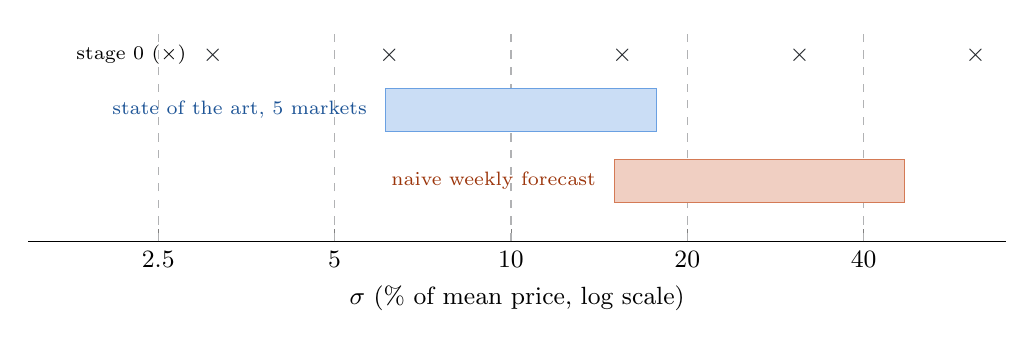
\begin{tikzpicture}
\begin{axis}[width=14cm, height=4.4cm, xmode=log, xmin=1.5, xmax=70, ymin=0, ymax=1.25, ytick=\empty,
  xtick={2.5,5,10,20,40}, xticklabels={2.5,5,10,20,40}, xlabel={$\sigma$ (\% of mean price, log scale)},
  axis y line=none, axis x line*=bottom, label style={font=\small}, tick label style={font=\small}, clip=false]
  \pgfplotsinvokeforeach{2.5,5,10,20,40}{\draw[ink!35, dashed] (axis cs:#1,0) -- (axis cs:#1,1.2);}
  \fill[accent!25, draw=accent!70] (axis cs:6.1,0.62) rectangle (axis cs:17.7,0.86);
  \node[font=\scriptsize, text=accent!70!black, anchor=east] at (axis cs:5.9,0.74) {state of the art, 5 markets};
  \fill[warn!25, draw=warn!70] (axis cs:15.0,0.22) rectangle (axis cs:47.0,0.46);
  \node[font=\scriptsize, text=warn!80!black, anchor=east] at (axis cs:14.5,0.34) {naive weekly forecast};
  \pgfplotsinvokeforeach{3.1,6.2,15.5,31.1,62.1}{\node[ink, font=\small] at (axis cs:#1,1.05) {$\times$};}
  \node[font=\scriptsize, anchor=east] at (axis cs:2.9,1.05) {stage 0 ($\times$)};
\end{axis}
\end{tikzpicture}
\end{center}
\textbf{Defence.} 2.5\% is better than any published model (it tests the small-error limit and continuity at
0); 5 and 10\% are best-in-class markets; 20\% is a typical market or a weaker model; 40\% is a naive
forecaster. The grid therefore spans from perfect information to no forecasting skill, with every published
value inside it. Precedent: Martinez-Rico et al.\ (2020), in a battery-bidding sensitivity analysis, use error
standard deviations of 0, 5, 10, 15 and 20\% (on renewable production, not price). The stage-0 values in
\$/MWh are inherited from the pilot so its results can be compared; they cover the same range.

\textbf{Caveat to state.} Real price errors are heavier-tailed than Gaussian: Lago et al.'s RMSE/MAE ratios
are 1.7--3.0, against 1.25 for a normal distribution. The Gaussian model is the maximum-entropy choice
for a given mean and variance and isolates the effect of size; the stage-3 bootstrap of real residuals
(\code{forecasts.bootstrap\_days}) is what captures spikes.

\subsection{Autocorrelation $\rho$: \{0, 0.5, 0.9\} between consecutive intervals}
\textbf{Anchor (own data).} Price forecast errors inherit the persistence of their drivers, above all the
wind forecast error. In the RTS-GMLC data of this project (\code{Data/timeseries\_hourly\_2020.csv}), the
day-ahead wind forecast error has autocorrelation 0.87 at 1\,h, 0.71 at 2\,h, \textbf{0.49 at 4\,h} and 0.23
at 8\,h; for PV, 0.73 / 0.49 / 0.22 / $-0.07$. An interval of the test case lasts 4\,h, so
$\rho\approx0.5$ is the data-anchored central value. $\rho=0$ (independent errors) is the lower bound;
$\rho=0.9$ is the hourly persistence of wind errors, i.e.\ the right value if the model is moved to hourly
resolution, or a forecast that is off by a near-constant amount all day. \emph{If $\Delta T$ changes, the
grid must be re-mapped}: the relevant quantity is the error's autocorrelation at lag $\Delta T$.

\subsection{Bias: \{$-10$, 0, $+10$\}\,\% of $\bar\lambda$}
A bias is a systematic level error: fuel or CO$_2$ prices moving after the model was trained, a regime the
training data did not contain. $\pm10\%$ is the same size as the state-of-the-art random error (6--18\%), so
the grid compares a systematic and a random error of equal magnitude; it is symmetric so that sign effects
can show up. One is built in: with the price floor, a negative bias is cut off in the zero-price intervals
(the forecast cannot go below 0), a positive one is not. The real bias is the mean residual of the stage-3
backtest. Two draws, one with more and one with less bias (notebook \S3); bottom row: the error split into
its bias (dashed) and random part:
\begin{center}
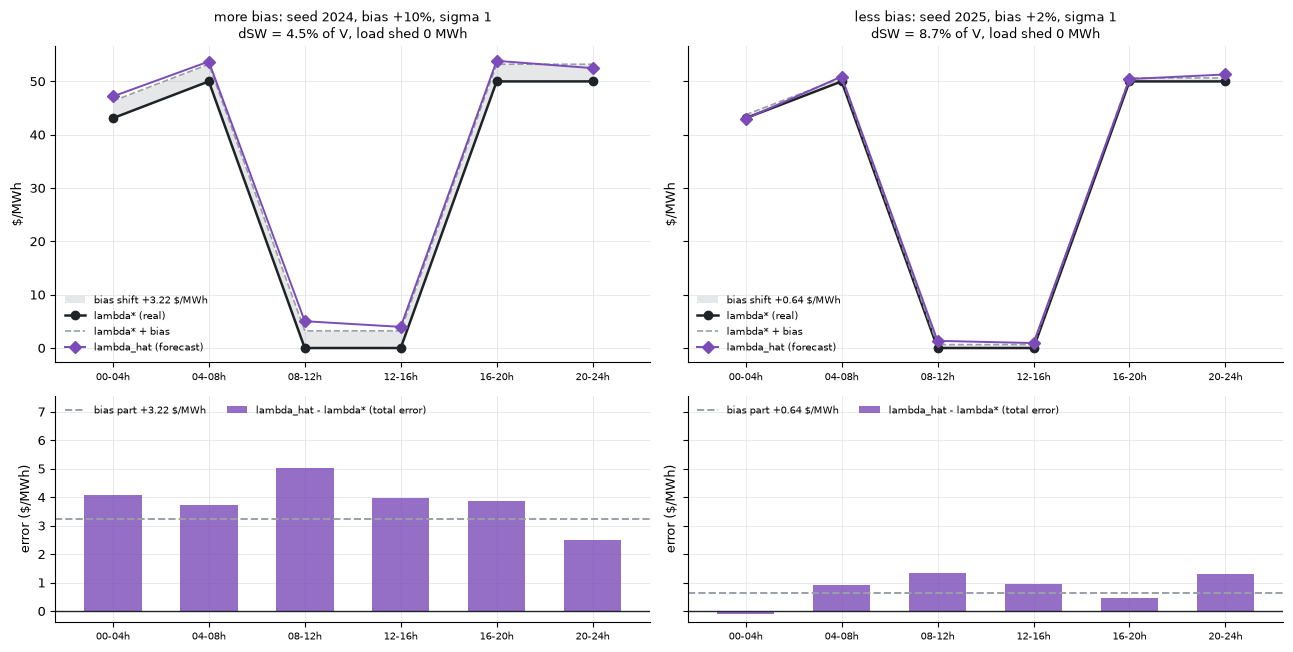
\includegraphics[width=0.9\textwidth]{figures/nb_bias.png}
\end{center}

\subsection{Common share $\omega$: \{0, 0.5, 1\} (stage 2, several batteries)}
$\omega=0$: each battery has its own forecaster, errors independent; $\omega=1$: all use the same forecast
(a common vendor or a public TSO forecast), so their errors move together; 0.5 the midpoint. These are the
two logical extremes; stage 3 estimates $\omega$ as the correlation between the residuals of two different
forecasters.

\subsection{Price floor $\underline\lambda=0$}
In the test system the cheapest supply is free, curtailable renewables and nobody bids below 0, so
$\lamstar_t\ge0$ always (here $\lamstar\in[0,50]$). A forecast below 0 predicts a price this market cannot
produce; a forecaster that knows the market's price range would not make it. The floor changes the error
distribution only where the true price is near 0: with $\lamstar_t=0$, the error becomes $\max(0,\sigma z)$,
zero half the time and $\sigma/\sqrt{2\pi}\approx0.40\,\sigma$ on average (an upward bias in those
intervals). \textbf{It matters a lot here:} without it, about 1 draw in 5 is catastrophic at every
$\sigma$ (Finding~2 in \S\ref{sec:poly}). Real markets can clear below zero (DK1 had 281 negative-price hours in 2023,
Forsyningstilsynet), driven by subsidies and inflexible generation; for a realistic stage-3 system the floor
must be set to that market's own minimum, or disabled. That is why it is a parameter, not a constant.

\subsection{Not error parameters, but chosen alongside them}
\begin{itemize}
  \item \textbf{Real-time premium $\psi$: \{0, 10, 50\}\,\$/MWh.} 0 is frictionless correction (lower bound on
    the loss). Martinez-Rico et al.\ (2020) apply imbalance penalties of 13--14\% of the price in the Iberian
    market, about 4.5\,\$/MWh at $\bar\lambda=32$; $\psi=10$ ($\approx31\%$ of $\bar\lambda$) is a conservative
    version of that, $\psi=50$ ($\approx155\%$) a scarcity stress test. Still an open decision with the
    supervisors (\code{experiments.md} \S8).
  \item \textbf{Draws $N$.} With the floor, the standard deviation of $\Delta SW\%$ within a setting is 3--5
    points (stage 0). The 95\% confidence half-width of a mean, $1.96\,s/\sqrt N$, is 0.5--0.8 points at
    $N=150$ and 0.3--0.4 at $N=500$ (stage 1): small enough to rank neighbouring grid points.
\end{itemize}

{\small\textbf{Sources.}
J.~Lago, G.~Marcjasz, B.~De~Schutter, R.~Weron, ``Forecasting day-ahead electricity prices: A review of
state-of-the-art algorithms, best practices and an open-access benchmark'', \emph{Applied Energy} 293 (2021)
116983, Table~3.
J.~Martinez-Rico et al., ``Forecast error sensitivity analysis for bidding in electricity markets with a hybrid
renewable plant using a battery energy storage system'', \emph{Sustainability} 12 (2020) 3577.
Forsyningstilsynet, \emph{The Danish Electricity and Natural Gas Markets 2023}.
RTS-GMLC time series, \code{Data/timeseries\_hourly\_2020.csv} (autocorrelations computed for this document).}

% =====================================================================
\section{Inside the multiplier polyhedron $\Pi$}
\label{sec:poly}
% =====================================================================

\subsection{What $\Pi$ is, in plain words}
To bid, the battery needs one number per interval: $\pi_t$, \textbf{the value of one stored MWh at the end
of interval $t$}. The bid follows from it (formula (E)): it will \emph{buy} at prices up to
$u_t=\alpha(\pi_t-\nuU_t)-\varepsilon$ (what a stored MWh is worth, minus losses) and \emph{sell} at prices
from $c_t=\zeta+\beta(\pi_t+\nuL_t)$ (what it gives up by selling it, plus losses). $\Pi$ is the set of all
$\pi$ (with the matching $\nu$) that are consistent with the prices and with the battery's own planned
schedule. Every point of $\Pi$ is a valid bid; the rule (\code{prelimit} or \code{solver}) picks one.
\begin{center}
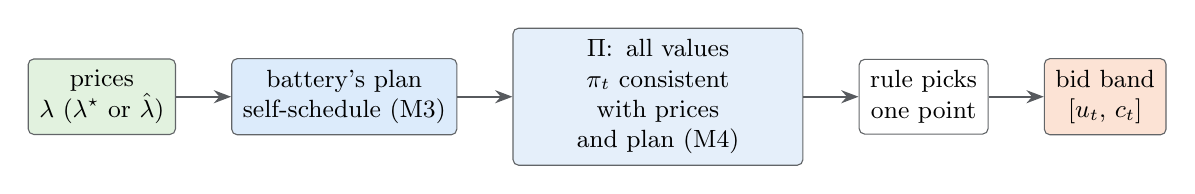
\begin{tikzpicture}[node distance=5mm and 7mm]
  \node[datbox] (p) {prices\\$\lambda$ ($\lamstar$ or $\lamhat$)};
  \node[box, fill=ex, right=of p] (s) {battery's plan\\self-schedule (M3)};
  \node[box, fill=accent!12, right=of s, text width=34mm] (P) {$\Pi$: all values $\pi_t$ consistent\\with prices and plan (M4)};
  \node[box, right=of P] (r) {rule picks\\one point};
  \node[box, fill=lp, right=of r] (b) {bid band\\$[u_t,\,c_t]$};
  \draw[arr] (p) -- (s); \draw[arr] (s) -- (P); \draw[arr] (P) -- (r); \draw[arr] (r) -- (b);
\end{tikzpicture}
\end{center}
\textbf{Why a set, not a single value.} Each $\pi_t$ is squeezed between two bounds, each set by a price
the battery reacted to in its plan: a stored MWh is worth \emph{at least} what it can still earn later (the
price at which the battery would sell it), and \emph{at most} what the battery passed up (the price at which it
chose not to buy more, or chose to sell rather than keep). Any value in between is consistent. If the two
prices give different numbers, $\pi_t$ has a range; if they give the same number, it is pinned. The state of
charge decides which prices bound which interval: $\pi$ can only change from one interval to the next when
the battery hits empty or full in between.

In the test system, at $\lamstar$: $\pi_2$ and $\pi_4$ lie anywhere in $[1.11,\,49]$\,\$/MWh, between refilling
with free energy at 08--16h ($(0+\varepsilon)/\alpha=1.11$) and selling at 16--24h ($(50-\zeta)/\beta=49$).
The others are pinned \emph{by ties} in $\lamstar$: $\pi_5$ is bounded by the prices at 16--20h and
20--24h, both 50; $\pi_1$ by buying at 00--04h, $(43.1+\varepsilon)/\alpha=49$, and selling at 04--08h,
$50-\zeta=49$ (a break-even round trip); $\pi_3$ by the two free intervals, both priced 0.

\textbf{How the pictures are made.} $\Pi$ lives in $\mathbb R^{3T}=\mathbb R^{18}$ and is unbounded in the
$\nu$ directions (at an hour where the plan does not charge, any less aggressive charge bid stays
consistent). Its $\pi$ part is bounded and is the part that matters, so the pictures show $\pi$. They are
exact: each point is an LP optimum over $\Pi$, and welfare is computed through \code{runner.evaluate\_blocks},
the same pipeline as the experiments, at $\psi=10$ (\code{scripts/plot\_multiplier\_polyhedron.py}).

\subsection{At the true prices: a square of choices, all equally good}
The battery's self-schedule at $\lamstar$ is \emph{not} Baldick's schedule: both are optimal for the battery
(Lemma~4), because $\lamstar$ makes it indifferent between them. The tie-breaker of M3 (\S\ref{sec:m3}) picks
the most active of the tied plans: charge 222\,MW at 00--04h and at 12--16h, discharge 200\,MW at 04--08h
and at 20--24h. That plan leaves the battery empty at the end of
04--08h and full at the end of 12--16h, so exactly two values are free, $\pi_2$ and $\pi_4$, each anywhere in
$[1.11,\,49]$; all others are pinned ($\pi_1=49$, $\pi_3=1.11$, $\pi_5=49$, $\pi_6=w=40$). $\Pi(\lamstar)$ is
therefore a \textbf{square}. Its corners include Baldick's own dual (A) and the two rules (B, C), and each
corner produces visibly different bids (yellow), for example a charge bid of 43.1 or 0\,\$/MWh at 04--08h:
\begin{center}
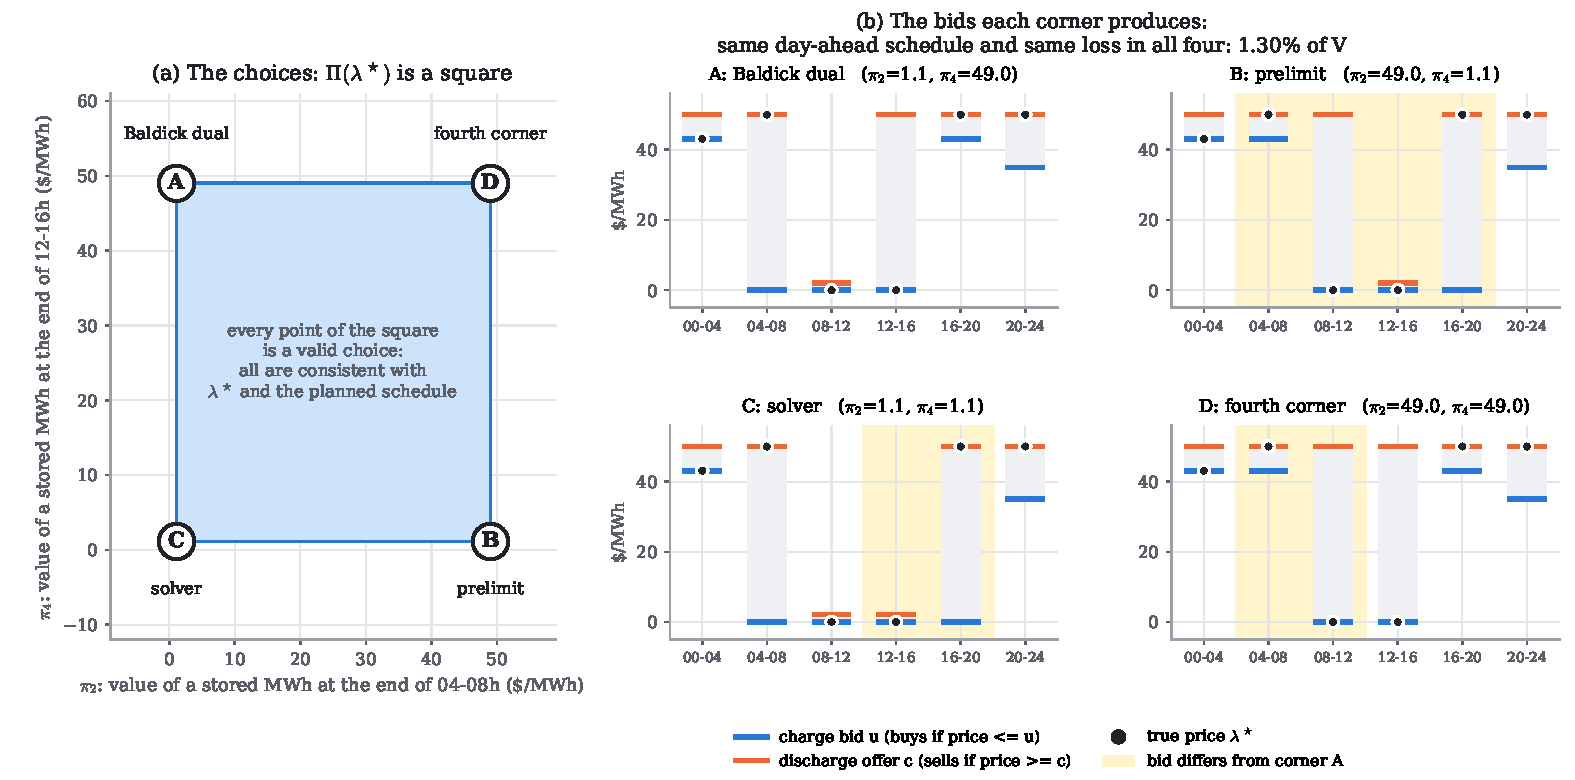
\includegraphics[width=\textwidth]{figures/fig_poly_true.pdf}
\end{center}
\textbf{Finding 1.} The four corners give \emph{exactly the same} day-ahead schedule (charge 100\,MW at
00--04h and 200\,MW at 12--16h; discharge 100\,MW at 04--08h, 75\,MW at 16--20h and 100\,MW at 20--24h), the
same prices and the same loss, 1.30\% of $V$. In every interval where their bids differ, the market price stays
on the same side of the bid, so the accepted quantities do not change. At $\lamstar$ the choice of rule is
therefore irrelevant: the whole \code{B\_star\_p} loss comes from the \emph{quantity plan} (which of the tied
optimal schedules the battery plans), not from the bid prices. Baldick's dual with Baldick's own quantities
(\code{B\_star}) gives 0.

\subsection{Under forecast error: the valid ranges move and open up}
A forecast breaks the ties of $\lamstar$ (prices of exactly 0 at 08--16h, a break-even round trip at
00--08h), so the battery's plan changes and with it the set of valid values. The clearest view is one
interval at a time: the range each $\pi_t$ can take, at the true prices and for 8 forecast draws:
\begin{center}
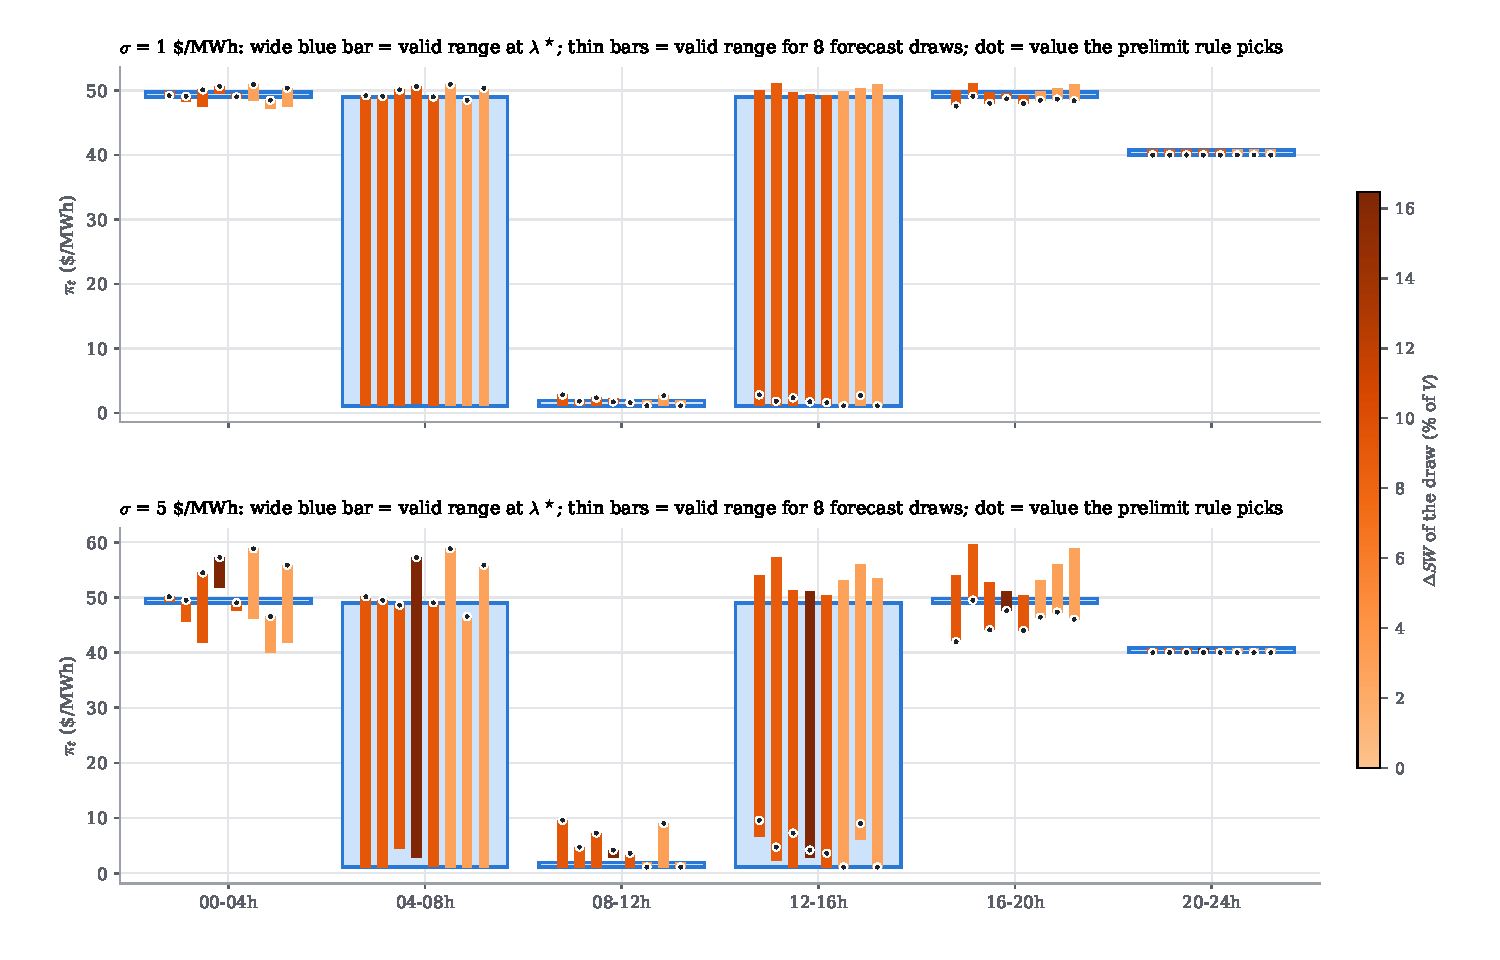
\includegraphics[width=\textwidth]{figures/fig_poly_ranges.pdf}
\end{center}
How to read it: at $\lamstar$ (wide blue bars) only 04--08h and 12--16h have freedom. Under a forecast the
ranges move, and the value the prelimit rule picks (dots) lands in different places, so the bids differ from
draw to draw; the colour of each draw is its loss. Intervals that were pinned open up (00--04h, 08--12h and
16--20h), because they were pinned only by ties in $\lamstar$: the two prices that bound them were exactly
equal (\S7.1). A forecast puts slightly different numbers on them, e.g.\ 52 at 16--20h and 48 at 20--24h
instead of 50 and 50, and the bounds separate by about that difference: $\pi_5\in[47,\,51]$ instead of
$\{49\}$. That is why the opened ranges are narrow at $\sigma=1$ and wider at $\sigma=5$. In full dimension, $\Pi(\lamhat)$ is 5-dimensional in 12 of these 16 draws and 4-dimensional in the 4 where
the floor clips both zero-price intervals to exactly 0, which restores one tie (exact 2-D and 3-D shadows of
it: \code{fig\_poly\_forecast.pdf} and \code{fig\_poly\_3d.pdf} in \code{docs/figures/}).

Per-draw $\Delta SW\%$ of the prelimit bid (price floor 0): $\sigma=1$: 9.3, 8.7, 9.3, 9.3, 9.3, 2.8, 3.1, 2.8;
\; $\sigma=5$: 9.3, 8.7, 9.3, 16.5, 9.3, 2.8, 3.1, 2.8. No draw sheds load.

\textbf{Finding 2: why the forecast is floored at 0.} Prices in this market cannot be negative (the cheapest
supply, curtailable renewables, is offered at 0), so the forecast is not allowed to be either:
$\lamhat_t\ge0$ (\code{ErrorModel.price\_floor = 0}). The floor matters because of the free intervals $t=3,4$,
where the true price is exactly 0. A charge block is accepted there only if its bid is $\ge0$, and the bid
follows the forecast ($u_t=\lamhat_t$ where the battery plans to charge). A negative forecast in both
intervals would make the battery buy nothing, reach the 16--20h shortfall empty, and force real time to shed
75\,MW at VOLL (mechanism traced step by step in the stage-0 notebook, Section~7). Because $\lamstar=0$
exactly there, an unbounded error would be negative with probability 1/2 whatever $\sigma$ is, so this
unphysical event would dominate every result. With the floor, the battery always buys the free energy and
the loss grows with $\sigma$. 200 seeds per $\sigma$ (seeds 1000--1199, prelimit, $\psi=10$):
\begin{center}\small
\begin{tabular}{@{}lccccc@{}}
\toprule
$\sigma$ (\$/MWh) & 1 & 2 & 5 & 10 & 20 \\
\midrule
mean $\Delta SW\%$ & 6.3 & 6.3 & 6.8 & 8.1 & 9.0 \\
\quad draws with load shed & 0 & 0 & 0 & 0 & 0 \\
\bottomrule
\end{tabular}
\end{center}
The tie-breaker of M3 never changes the plan in these 1\,000 draws. Load shedding is rare but not
impossible: none of seeds 1000--2999 at $\sigma=20$ sheds, but it can happen when the floor clips several
intervals at once, e.g.\ for the forecast $\lamhat=(0,\,0,\,1.2,\,0,\,32,\,48.3)$. There the floor clips three intervals
to exactly 0, the battery is indifferent \emph{when} to charge, and it plans to buy at 00--04h (true price
43.1), where the market lets it take only 100\,MW. It runs empty by 16--20h and 75\,MW is shed. This is a
timing tie, which throughput cannot break (\S\ref{sec:m3}).

The remaining sensitivity to near-ties in this small case (losses jump between a few discrete values, 2.8, 3.1,
8.7, 9.3, 16.5\,\%) is a property of the test system, not of the design. The tie-breaker removes the
\emph{exact} ties of the $\sigma=0$ plan, but a forecast error turns them into \emph{near}-ties that the error
itself decides, in a random direction. A case without near-ties, or the block-cost perturbation of
\code{CLAUDE.md}~\S7, should make the loss grow continuously with $\sigma$.

% =====================================================================
\section{One experiment draw, end to end}
% =====================================================================

\begin{center}
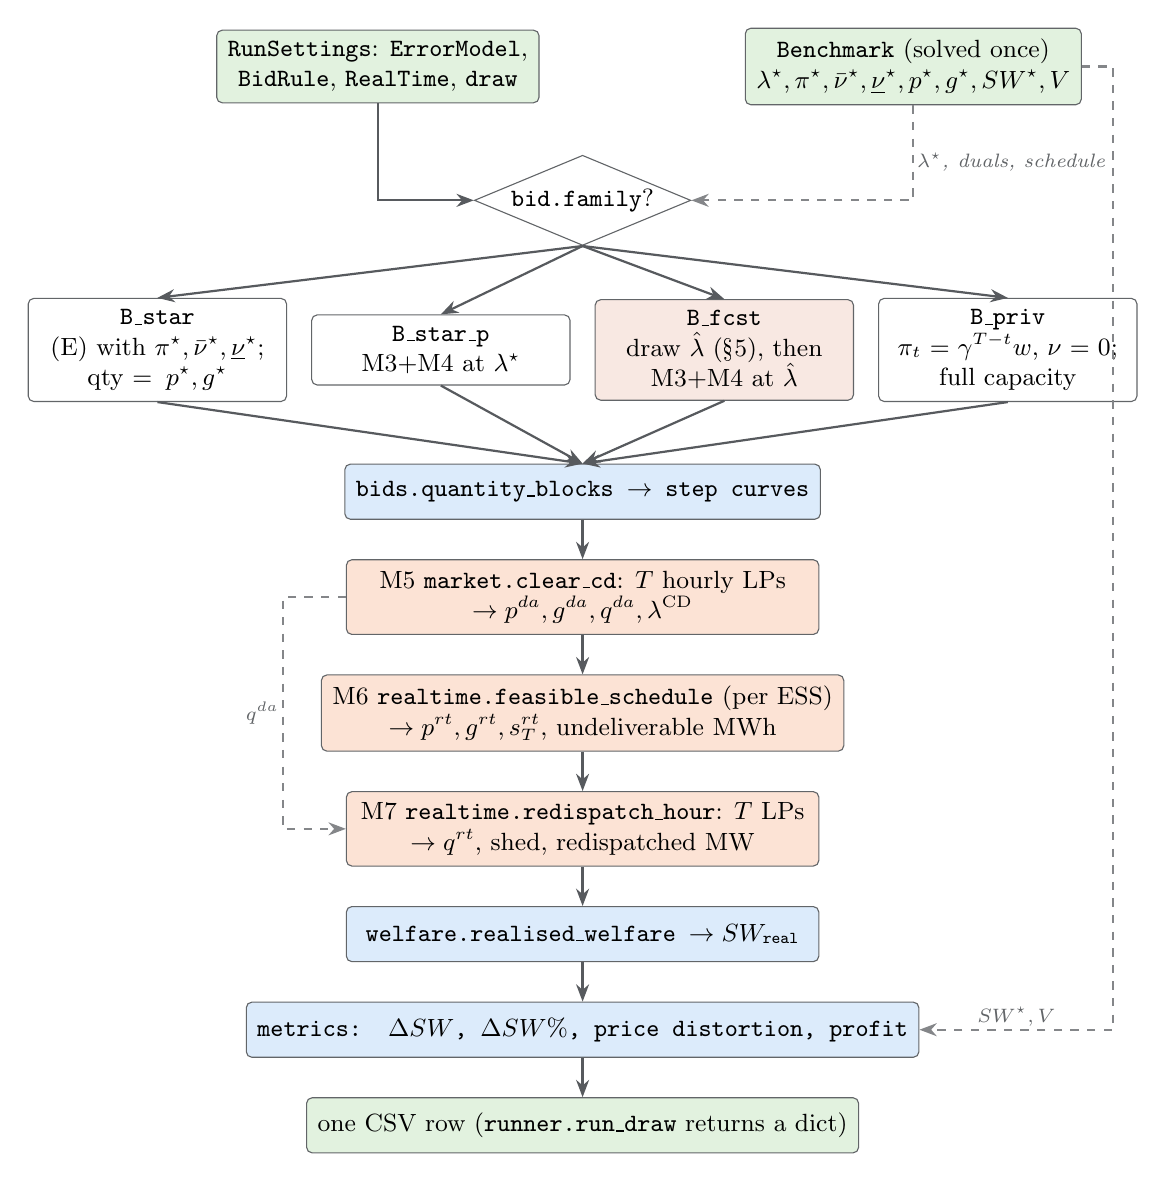
\begin{tikzpicture}[node distance=5mm]
  \node[datbox] (set) at (-2.6,0) {\code{RunSettings}: \code{ErrorModel},\\\code{BidRule}, \code{RealTime}, \code{draw}};
  \node[datbox] (bench) at (4.2,0) {\code{Benchmark} (solved once)\\$\lamstar,\pi^\star,\nuU^\star,\nuL^\star,p^\star,g^\star,SW^\star,V$};
  \node[dec] (fam) at (0,-1.7) {\code{bid.family}?};
  \node[box, text width=3.0cm] (b1) at (-5.4,-3.6) {\code{B\_star}\\(E) with $\pi^\star,\nuU^\star,\nuL^\star$;\\ qty $=p^\star,g^\star$};
  \node[box, text width=3.0cm] (b2) at (-1.8,-3.6) {\code{B\_star\_p}\\M3+M4 at $\lamstar$};
  \node[box, text width=3.0cm, fill=warn!12] (b3) at (1.8,-3.6) {\code{B\_fcst}\\draw $\lamhat$ (\S5), then\\M3+M4 at $\lamhat$};
  \node[box, text width=3.0cm] (b4) at (5.4,-3.6) {\code{B\_priv}\\$\pi_t=\gamma^{T-t}w$, $\nu=0$;\\full capacity};
  \node[mod, minimum width=60mm] (qb) at (0,-5.4) {bids.quantity\_blocks $\to$ step curves};
  \node[lpbox, below=of qb, minimum width=60mm] (m5) {M5 \code{market.clear\_cd}: $T$ hourly LPs\\$\to p^{da}, g^{da}, q^{da}, \lambda^{\text{CD}}$};
  \node[lpbox, below=of m5, minimum width=60mm] (m6) {M6 \code{realtime.feasible\_schedule} (per ESS)\\$\to p^{rt}, g^{rt}, s^{rt}_T$, undeliverable MWh};
  \node[lpbox, below=of m6, minimum width=60mm] (m7) {M7 \code{realtime.redispatch\_hour}: $T$ LPs\\$\to q^{rt}$, shed, redispatched MW};
  \node[mod, below=of m7, minimum width=60mm] (wf) {welfare.realised\_welfare $\to SW_{\text{real}}$};
  \node[mod, below=of wf, minimum width=60mm] (mt) {metrics: $\Delta SW$, $\Delta SW\%$, price distortion, profit};
  \node[datbox, below=of mt, minimum width=60mm] (row) {one CSV row (\code{runner.run\_draw} returns a dict)};
  \foreach \b in {b1,b2,b3,b4} { \draw[arr] (fam.south) -- (\b.north); \draw[arr] (\b.south) -- (qb.north); }
  \draw[arr] (set.south) |- (fam.west);
  \draw[arr] (qb) -- (m5); \draw[arr] (m5) -- (m6); \draw[arr] (m6) -- (m7); \draw[arr] (m7) -- (wf);
  \draw[arr] (wf) -- (mt); \draw[arr] (mt) -- (row);
  \draw[darr] (bench.south) |- node[lab, pos=0.3, right]{$\lamstar$, duals, schedule} (fam.east);
  \draw[darr] (bench.east) -- ++(4mm,0) |- node[lab, pos=0.75, above]{$SW^\star, V$} (mt.east);
  \draw[darr] (m5.west) -- ++(-8mm,0) |- node[lab, pos=0.25, left]{$q^{da}$} (m7.west);
\end{tikzpicture}
\end{center}

\textbf{Around the draw} (\code{runner.run\_all}): for each \code{RunSettings} in the list from
\code{config}, skip if \code{results/<stage>/} \code{<setting\_id>.csv} exists (resume), else call
\code{run\_setting} (= \code{run\_draw} for \code{draw}$=0..$\code{draws}$-1$), write the CSV, and finally
\code{meta.json} (date, git commit, versions, $SW^\star$, $SW_{\text{noESS}}$, $V$, $\lamstar$).
Inside \code{run\_draw}, everything from day-ahead clearing to welfare (M5--M7 and welfare) is one function,
\code{runner.evaluate\_blocks}, which takes the case, the bid blocks and the real-time settings and returns an
\code{Outcome} with every intermediate result. Any bid curve can therefore be scored through the identical
pipeline, and inspected step by step (\S\ref{sec:see}).

\textbf{Cost per draw} (\code{B\_fcst}, one battery, $T=6$): 1 (M3) + 12 (\code{pi\_range}, M4) + 6 (M5)
+ 1 (M6) + 6 (M7) = 26 small LPs with \code{"prelimit"}; 15 with \code{"solver"} (one vertex LP instead of
\code{pi\_range}).

\subsection{What each bid family isolates}
\begin{center}\small
\begin{tabular}{@{}lllll@{}}
\toprule
Family & Prices from & Quantity plan & Role & Expected $\Delta SW$ \\
\midrule
\code{B\_star} & $\lamstar$, Baldick's own duals & benchmark $(p^\star,g^\star)$ & gate: equivalence holds & $0$ \\
\code{B\_star\_p} & $\lamstar$, M4 selection & own self-schedule at $\lamstar$ & cost of selecting from $\Pi$ & $\ge 0$ \\
\code{B\_fcst} & $\lamhat_e$, M4 selection & own self-schedule at $\lamhat_e$ & \textbf{main experiment} & $\ge$ \code{B\_star\_p} \\
\code{B\_priv} & none: $\pi_t=\gamma^{T-t}w$ & full capacity & lower bound (technical data only) & reference \\
\bottomrule
\end{tabular}
\end{center}

% =====================================================================
\section{Seeing each step: notebook, explorer and albums}
\label{sec:see}
% =====================================================================

Every box of the pipeline above has a picture in \code{notebooks/stage0\_experiments.ipynb}. The notebook
follows the model's order, so it can be read side by side with this document:
\begin{center}
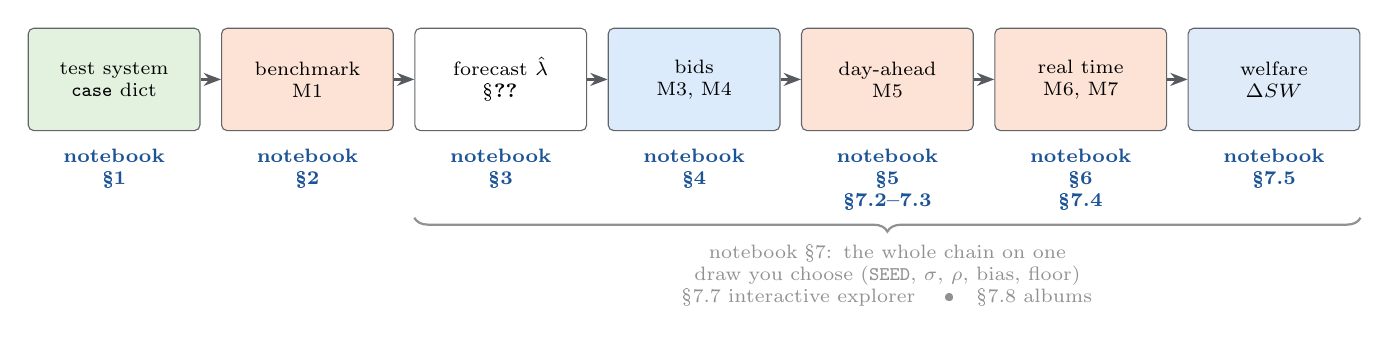
\begin{tikzpicture}[
  st/.style={box, minimum width=20mm, minimum height=13mm, text width=19mm, font=\scriptsize},
  nb/.style={font=\scriptsize\bfseries, text=accent!70!black},
  node distance=2.6mm]
  \node[st, fill=dat] (s1) {test system\\\code{case} dict};
  \node[st, fill=lp, right=of s1] (s2) {benchmark\\M1};
  \node[st, fill=white, right=of s2] (s3) {forecast $\lamhat$\\\S\ref{sec:values}};
  \node[st, fill=ex, right=of s3] (s4) {bids\\M3, M4};
  \node[st, fill=lp, right=of s4] (s5) {day-ahead\\M5};
  \node[st, fill=lp, right=of s5] (s6) {real time\\M6, M7};
  \node[st, fill=accent!15, right=of s6] (s7) {welfare\\$\Delta SW$};
  \foreach \a/\b in {s1/s2, s2/s3, s3/s4, s4/s5, s5/s6, s6/s7} \draw[arr] (\a) -- (\b);
  \foreach \n/\t in {s1/{\S1}, s2/{\S2}, s3/{\S3}, s4/{\S4}, s5/{\S5\\\S7.2--7.3}, s6/{\S6\\\S7.4}, s7/{\S7.5}}
    \node[nb, below=1mm of \n, align=center, text width=19mm] {notebook\\\t};
  \draw[decorate, decoration={brace, amplitude=5pt, mirror}, thick, ink!50]
    ([yshift=-11mm]s3.south west) -- ([yshift=-11mm]s7.south east)
    node[midway, below=6pt, font=\scriptsize, align=center, text width=95mm]
    {notebook \S7: the whole chain on one draw you choose (\code{SEED}, $\sigma$, $\rho$, bias, floor)\\
     \S7.7 interactive explorer \quad\textbullet\quad \S7.8 albums};
\end{tikzpicture}
\end{center}
\textbf{Interactive explorer (notebook \S7.7).} Widgets for the seed, $\sigma$, $\rho$, bias, price floor,
bid rule and $\psi$; every change re-solves one draw (about 0.03\,s) and redraws eight panels: (a) the
forecast error, (b) forecast, bid bands and prices, (c) day-ahead dispatch, (d) SOC feasibility, (e) sold vs.\
delivered, (f) redispatch and shedding, (g) real-time dispatch, (h) where the loss comes from, cost by cost. A
status line says whether the last change moved the dispatch; a play control steps one parameter through its
range.

\textbf{Albums (notebook \S7.8, and the standalone page \code{docs/figures/album\_seed1036.html}).} For one
error shape $z$ (one seed), one album per parameter ($\sigma$, $\rho$, bias, $\psi$, floor, rule), each picture
rendered in advance and browsed with a labelled slider; panel (h) becomes the loss along the slider. One
picture of the $\sigma$ album:
\begin{center}
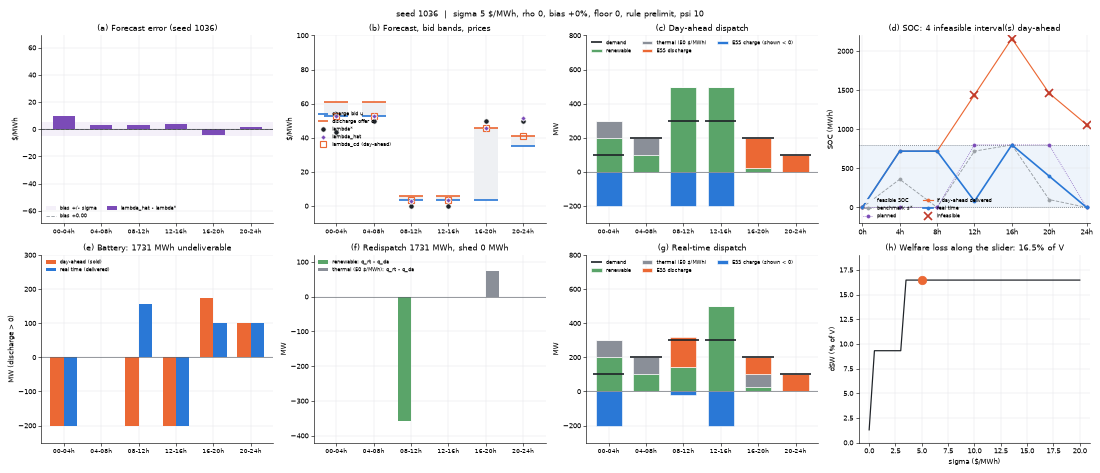
\includegraphics[width=\textwidth]{figures/nb_explorer.png}
\end{center}
{\small What to take from it: with $z$ fixed, $\lamhat$ moves \emph{continuously} with $\sigma$, $\rho$ and
the bias, but the market outcome moves in \emph{steps}, because the battery's schedule only changes when the
forecast crosses a decision threshold. At $\sigma=1$\,\$/MWh, 40 seeds give only 8 distinct day-ahead battery
schedules (15 at $\sigma\ge5$); a $\sigma$ sweep at a fixed seed crosses at most two thresholds in this
test system.}

% =====================================================================
\section{Configuration and stages (\code{config.py})}
% =====================================================================

\begin{center}
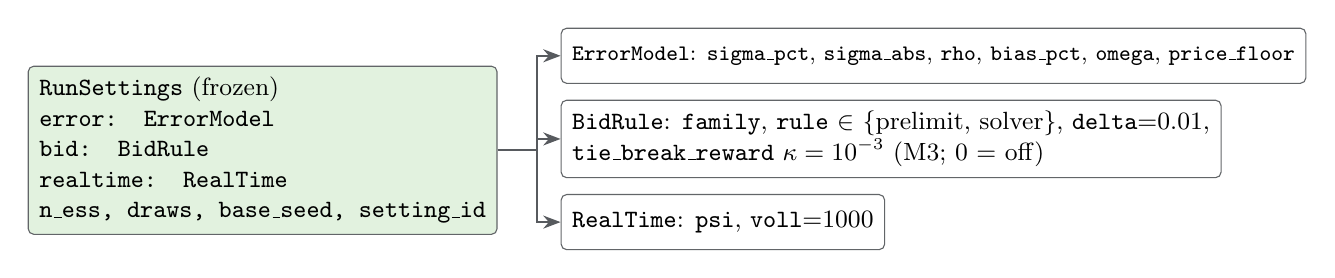
\begin{tikzpicture}[node distance=4mm]
  \node[datbox, align=left] (rs) {\textbf{\code{RunSettings}} (frozen)\\
    \code{error: ErrorModel}\\\code{bid: BidRule}\\\code{realtime: RealTime}\\\code{n\_ess, draws, base\_seed, setting\_id}};
  \node[box, align=left, right=8mm of rs, yshift=12mm, font=\footnotesize] (em) {\code{ErrorModel}: \code{sigma\_pct}, \code{sigma\_abs}, \code{rho}, \code{bias\_pct}, \code{omega}, \code{price\_floor}};
  \node[box, align=left, below=2mm of em.south west, anchor=north west] (br) {\code{BidRule}: \code{family}, \code{rule} $\in$ \{prelimit, solver\}, \code{delta}=0.01,\\\code{tie\_break\_reward} $\kappa=10^{-3}$ (M3; 0 = off)};
  \node[box, align=left, below=2mm of br.south west, anchor=north west] (rt) {\code{RealTime}: \code{psi}, \code{voll}=1000};
  \draw[arr] (rs.east) -- ++(5mm,0) |- (em.west);
  \draw[arr] (rs.east) -- ++(5mm,0) |- (br.west);
  \draw[arr] (rs.east) -- ++(5mm,0) |- (rt.west);
\end{tikzpicture}
\end{center}

\begin{center}\small
\begin{tabularx}{\textwidth}{@{}l>{\raggedright\arraybackslash}X>{\raggedright\arraybackslash}p{3.6cm}@{}}
\toprule
Stage & Grid & Status \\
\midrule
0 (gate) & \code{B\_star}; \code{B\_priv} at $\psi\in\{0,10,50\}$; \code{B\_star\_p}, \code{B\_fcst} at $\sigma\in\{0,1,2,5,10,20\}$ \$/MWh, $\rho=0$, $\psi=10$, prelimit, 150 draws & 16 settings, 1\,506 draws: \textbf{run} \\
1 & \code{B\_fcst}: $\sigma\%\in\{0,2.5,5,10,20,40\}\times\rho\in\{0,0.5,0.9\}\times$ bias $\in\{-10,0,10\}\%\times$ rule $\times\ \psi\in\{0,10,50\}$ = 324 settings, 500 draws & defined, not run \\
2 & fleet of 5--20 batteries, 10--40\% of peak; $\rho\in\{0,0.9\}$, $\omega\in\{0,0.5,1\}$ & blocked: \code{fleet\_case} raises \\
3 & realistic system + calibrated/empirical errors & \code{bootstrap\_days} stub \\
\bottomrule
\end{tabularx}
\end{center}

% =====================================================================
\section{Verification layer}
% =====================================================================

\begin{center}
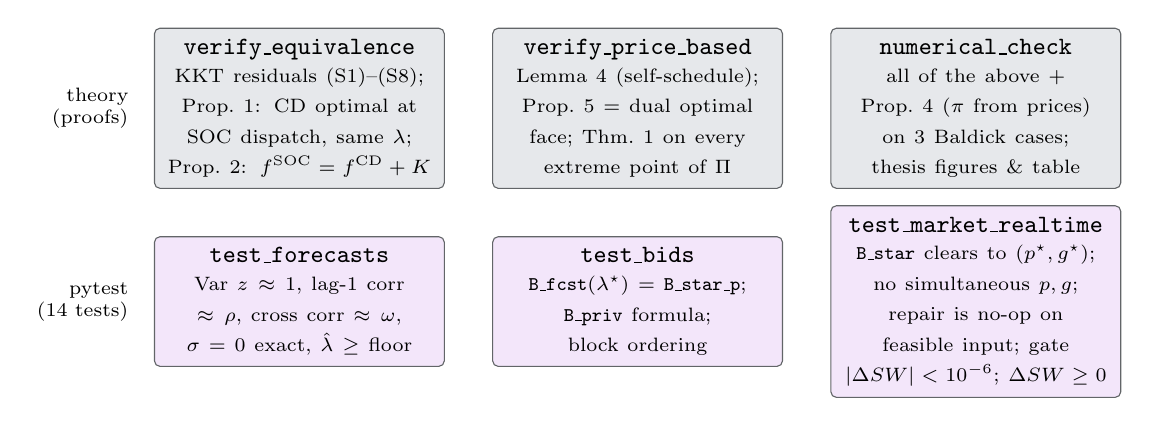
\begin{tikzpicture}[node distance=3mm and 6mm]
  \node[romod, text width=3.4cm] (v1) {verify\_equivalence\\[-1pt]\scriptsize\rmfamily KKT residuals (S1)--(S8); Prop.~1: CD optimal at SOC dispatch, same $\lambda$; Prop.~2: $f^{\text{SOC}}=f^{\text{CD}}+K$};
  \node[romod, text width=3.4cm, right=of v1] (v2) {verify\_price\_based\\[-1pt]\scriptsize\rmfamily Lemma~4 (self-schedule); Prop.~5 = dual optimal face; Thm.~1 on every extreme point of $\Pi$};
  \node[romod, text width=3.4cm, right=of v2] (v3) {numerical\_check\\[-1pt]\scriptsize\rmfamily all of the above + Prop.~4 ($\pi$ from prices) on 3 Baldick cases; thesis figures \& table};
  \node[drvbox, text width=3.4cm, below=6mm of v1] (t1) {test\_forecasts\\[-1pt]\scriptsize\rmfamily Var $z\approx1$, lag-1 corr $\approx\rho$, cross corr $\approx\omega$, $\sigma=0$ exact, $\lamhat\ge$ floor};
  \node[drvbox, text width=3.4cm, right=of t1] (t2) {test\_bids\\[-1pt]\scriptsize\rmfamily \code{B\_fcst}($\lamstar$) = \code{B\_star\_p}; \code{B\_priv} formula; block ordering};
  \node[drvbox, text width=3.4cm, right=of t2] (t3) {test\_market\_realtime\\[-1pt]\scriptsize\rmfamily \code{B\_star} clears to $(p^\star,g^\star)$; no simultaneous $p,g$; repair is no-op on feasible input; gate $|\Delta SW|<10^{-6}$; $\Delta SW\ge0$};
  \node[left=2mm of v1, font=\scriptsize, align=right] {theory\\(proofs)};
  \node[left=2mm of t1, font=\scriptsize, align=right] {pytest\\(14 tests)};
\end{tikzpicture}
\end{center}

% =====================================================================
\section{Numbers: benchmark and stage 0}
\label{sec:numbers}
% =====================================================================

\begin{center}
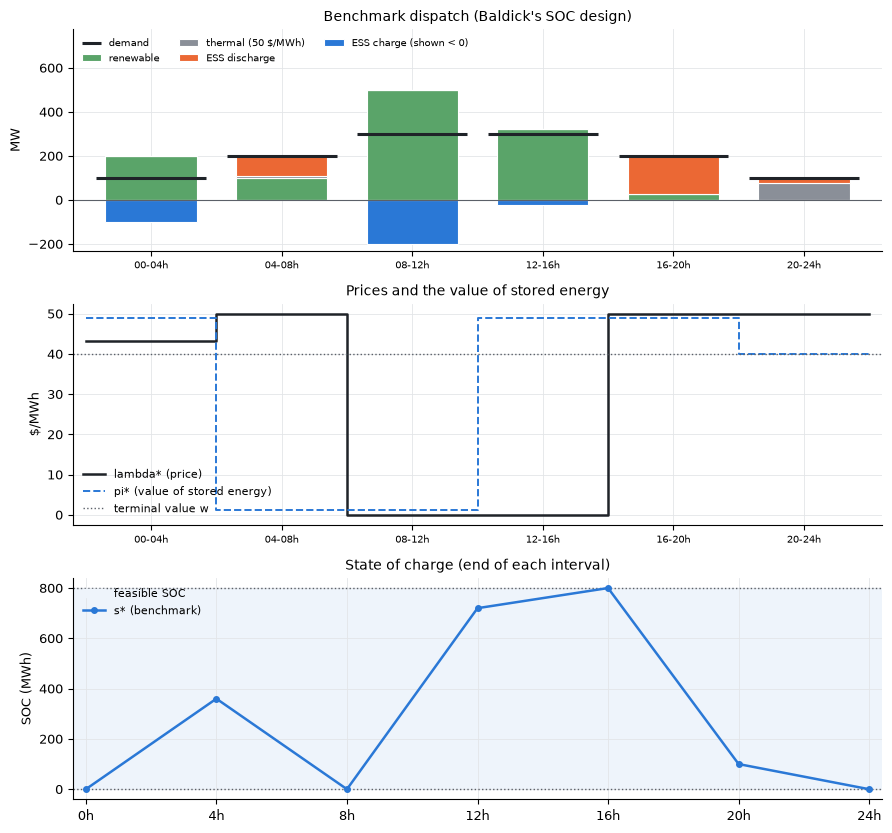
\includegraphics[width=0.72\textwidth]{figures/nb_benchmark.png}\\[2pt]
{\footnotesize Baldick's benchmark (notebook \S2): dispatch, prices $\lamstar$ against the value of stored
energy $\pi^\star$, and the SOC path.}\\[6pt]

\small
\begin{tabular}{@{}lrrrrrr@{}}
\toprule
$t$ & 1 & 2 & 3 & 4 & 5 & 6\\
\midrule
$\lamstar_t$ & 43.1 & 50 & 0 & 0 & 50 & 50\\
$s^\star_t$ & 360 & 0 & 720 & 800 & 100 & 0\\
$\pi^\star_t$ & 49 & 1.1 & 1.1 & 49 & 49 & 40\\
$\nuU^\star_t$ & 0 & 0 & 0 & 47.9 & 0 & 0\\
$\nuL^\star_t$ & 0 & 47.9 & 0 & 0 & 0 & 9\\
\bottomrule
\end{tabular}\qquad
$SW^\star=-19\,449$, \ $SW_{\text{noESS}}=-360\,000$, \ $V = 340\,551$ \$/day.
\end{center}

\medskip
$V$ is dominated by reliability: without the battery, interval 5 has a 75 MW shortfall
(25 MW renewable + 100 MW thermal vs.\ 200 MW demand) shed at VOLL for 4 h ($=300\,000$\,\$).
$\lamstar_1 = 43.1 = a\,\pi_1-\varepsilon$: the battery is the marginal unit there.

\begin{center}\small
\begin{tabular}{@{}lrrrrrr@{}}
\toprule
Setting (stage 0, price floor 0) & draws & mean $\Delta SW\%$ & sd & median & p95 & undeliverable MWh\\
\midrule
\code{B\_star} & 1 & 0.00 & & 0.00 & 0.00 & 0\\
\code{B\_star\_p} (any $\sigma$) & 1/150 & 1.30 & 0 & 1.30 & 1.30 & 40\\
\code{B\_fcst}, $\sigma=0$ & 1 & 1.30 & & 1.30 & 1.30 & 40\\
\code{B\_fcst}, $\sigma=1$ & 150 & 5.80 & 3.10 & 4.47 & 9.31 & 976\\
\code{B\_fcst}, $\sigma=2$ & 150 & 5.80 & 3.10 & 4.47 & 9.31 & 976\\
\code{B\_fcst}, $\sigma=5$ & 150 & 6.22 & 3.68 & 4.47 & 9.31 & 1\,002\\
\code{B\_fcst}, $\sigma=10$ & 150 & 7.11 & 4.64 & 7.49 & 16.46 & 1\,050\\
\code{B\_fcst}, $\sigma=20$ & 150 & 7.85 & 4.88 & 8.22 & 16.46 & 1\,091\\
\code{B\_priv}, $\psi=0/10/50$ & 1 & 0.00 / 3.09 / 15.43 & & & & 1\,051\\
\bottomrule
\end{tabular}
\end{center}
Reading: the gate passes (\code{B\_star} gives $\Delta SW=0$). At zero error, building the bid from the
tie-broken self-schedule and a selected point of $\Pi$ costs 1.30\% of $V$ (\S\ref{sec:m3}, Finding~1). As soon as there is any error the mean jumps to about 6\%, and it rises
with $\sigma$ to 7.9\% at 20\,\$/MWh. No draw of this run sheds load. The jump from 1.3 to 6\% is the cost of
\emph{near}-indifference: at $\sigma=0$ the tie-breaker picks a good plan, but a forecast error of 1\,\$/MWh
already makes the battery strictly prefer one of the tied plans, chosen by the sign of the error. The
tie-breaker changes the plan in none of the 750 forecast draws: under forecast error there are no exact ties
left for it to break. \code{B\_priv} at $\psi=10$ (3.1\%) still beats \code{B\_fcst} on average here.

\textbf{Paired comparison (common random numbers, \S\ref{sec:crn}).} All rows use the same 150 error shapes,
so neighbouring error sizes can be compared draw by draw (\code{metrics.paired\_difference}; difference = loss at
the larger $\sigma$ minus loss at the smaller):
\begin{center}\small
\begin{tabular}{@{}lccccc@{}}
\toprule
step in $\sigma$ (\$/MWh) & mean difference & 95\% CI & half-width, paired & half-width, unpaired & draws not lower\\
\midrule
$1\to2$ & 0.00 & $[0.00,\,0.00]$ & 0.00 & 0.70 & 100\%\\
$2\to5$ & 0.42 & $[0.13,\,0.70]$ & 0.29 & 0.77 & 99\%\\
$5\to10$ & 0.90 & $[0.53,\,1.27]$ & 0.37 & 0.95 & 100\%\\
$10\to20$ & 0.74 & $[0.39,\,1.09]$ & 0.35 & 1.08 & 99\%\\
\bottomrule
\end{tabular}
\end{center}
The paired intervals are 2.5--3 times narrower, so every step from $\sigma=2$ upwards is resolved: a larger
error costs more. In 146 of the 150 draws the loss never decreases as $\sigma$ grows. In 99 of them it is the
\emph{same} at every $\sigma$: the \emph{shape} of the error decides the battery's plan, and its size rarely
does. That is also why $\sigma=1$ and 2 give identical losses in every draw. These are the numbers in
\code{results/stage0/*.csv}; the notebook reproduces them exactly, in any session.

% =====================================================================
\section{Notation crosswalk}
% =====================================================================

\begin{center}\small
\begin{tabular}{@{}llll@{}}
\toprule
Meaning & Code (\code{case["ess"]}) & Thesis / \code{experiments.md} & Root \code{CLAUDE.md} \\
\midrule
charge efficiency (energy in per MWh bought) & \code{a} & $\alpha$ & $\alpha$ \\
discharge factor (energy out per MWh sold) & \code{b} & $\beta$ & $1/\beta$ \textcolor{warn}{(!)} \\
self-discharge retention & \code{g} & $\gamma$ & -- \\
charge / discharge cost & \code{eps}, \code{zet} & $\varepsilon$, $\zeta$ & $\varepsilon$, $\zeta$ \\
charge / discharge power & \code{p}, \code{g} (LP vars) & $p$, $g$ & $c$, $d$ \\
SOC limits, initial SOC & \code{smin}, \code{smax}, \code{s0} & $\underline s,\bar s,s_0$ & $\bar S$, $s_0$ \\
power limits & \code{pbar}, \code{gbar} & $\bar p$, $\bar g$ & $\bar C$, $\bar D$ \\
terminal value (linear) & \code{w} & $w$, $b(s_T)=w s_T$ & $b(s_T)$ \\
SOC dual (value of stored energy) & \code{y["pi",e,t]} & $\pi_t$ & $\mu_t$ \\
SOC-limit duals & \code{nuU}, \code{nuL} & $\nuU$, $\nuL$ & -- \\
charge bid / discharge offer & \code{u}, \code{c} & $u$, $c$ & $\pi^{\text{bid}}$, $\pi^{\text{offer}}$ \\
\bottomrule
\end{tabular}
\end{center}
{\small The root \code{CLAUDE.md} brief (RTS-GMLC data, \code{dp.py}, \code{curves.py}, milestones M1--M6)
describes the earlier framework now in \code{Archive/guide\_md\_framework/}; it is \emph{not} the code
documented here. In particular its $\beta$ divides discharge, whereas the code's \code{b} multiplies it.}

% =====================================================================
\section{Caveats found while reading the code}
% =====================================================================

\begin{enumerate}
  \item \textbf{Common error component breaks with several batteries.} \code{run\_draw} calls
    \code{forecast\_prices(..., n\_ess, ...)} \emph{inside} the per-battery loop and keeps row \code{e}, so
    $\chi$ is redrawn for every battery and the cross-battery correlation is no longer $\omega$. Harmless for
    $n_{\text{ess}}=1$ (stages 0--1); must be fixed before stage 2 (draw once, before the loop).
  \item \textbf{\code{B\_star\_p} ignores $\sigma$}, so the five stochastic \code{B\_star\_p} settings in
    stage 0 are 750 identical draws (all 1.30\%).
  \item \textbf{Hourly clearing assumes no binding ramps.} \code{market.clear\_cd} solves each hour alone;
    a system with binding ramps or a network needs a multi-hour version.
  \item \textbf{Test system is the substitute \code{baldick\_case}}, not the pilot \code{day\_case}
    (\code{pilot/} is absent), so the published pilot numbers cannot be matched, and $V$ mostly reflects avoided
    shedding.
\end{enumerate}

\end{document}
